\documentclass{amsart}

\usepackage{amsmath,amsfonts,amsthm,amssymb,stmaryrd,paralist,tikz,amsthm}
\usepackage[mathscr]{euscript}
\usetikzlibrary{matrix,arrows,decorations.pathmorphing}



\newcommand{\R}{\mathbb{R}}
\newcommand{\Q}{\mathbb{Q}}
\newcommand{\Z}{\mathbb{Z}}
\newcommand{\C}{\mathbb{C}}
\newcommand{\N}{\mathbb{N}}
\newcommand{\D}{\mathbb{D}}
\newcommand{\T}{\mathbb{T}}
\newcommand{\RP}{\mathbb{R}\mathrm{P}}
\newcommand{\CP}{\mathbb{C}\mathrm{P}}
\renewcommand{\H}{\mathbb{H}}
\let\oldS\S
\renewcommand{\S}{\mathbb{S}}
\newcommand{\s}{\mathbb{S}}


\newtheorem{thm}{Theorem}[section]
\newtheorem*{thm*}{Theorem}
\newtheorem{lem}[thm]{Lemma}
\newtheorem*{lem*}{Lemma}
\newtheorem{cor}[thm]{Corollary}
\newtheorem*{cor*}{Corollary}
\newtheorem{prop}[thm]{Proposition}
\newtheorem*{prop*}{Proposition}
\newtheorem{defn}{Definition}
\newtheorem*{defn*}{Definition}
\newtheorem{question}{Question}
\newtheorem*{question*}{Question}
\newtheorem{conj}{Conjecture}
\newtheorem*{conj*}{Conjecture}

\newtheorem{bigthm}{Theorem}
\renewcommand{\thebigthm}{\Alph{bigthm}}

\newcommand{\re}{\mathrm{Re}}
\newcommand{\im}{\mathrm{Im}}
\newcommand{\iprod}[1]{\left< #1 \right>}
\newcommand{\abs}[1]{\left| #1 \right|}
\newcommand{\set}[1]{\left\{ #1 \right\} }
\newcommand{\norm}[1]{ \left\| #1 \right\| }
\newcommand{\del}{\nabla}
\newcommand{\two}{I\!\!I}


\usepackage{fancyhdr}
 \pagestyle{fancy}
 \chead{\sf DRAFT VERSION 5 --- {\today}}
 \setlength{\headheight}{14pt}
 \setlength{\footskip}{0.5in}
 \lhead{} \rhead{} \lfoot{} \cfoot{\thepage} \rfoot{}
 \renewcommand{\headrulewidth}{0pt}
 \renewcommand{\footrulewidth}{0pt}



\usepackage{color}
\definecolor{verydarkblue}{rgb}{0,0,0.4}
\usepackage{hyperref}
\hypersetup{
pdfauthor={Keaton Quinn},
pdftitle={Asymptotically Poincar\'e surfaces in quasi-Fuchsian manifolds},
colorlinks=true,linkcolor=verydarkblue,
citecolor=verydarkblue,urlcolor=verydarkblue
}



\begin{document}

\title{Limits of foliations \\ in quasi-Fuchsian manifolds}

\author{Keaton Quinn}

\maketitle

\begin{center} {\sf DRAFT VERSION 5 --- {\today} } \end{center}

\begin{abstract}
We study the asymptotic behavior of certain foliations of ends of quasi-Fuchsian manifolds. 
We introduce a class of such foliations, which we call asymptotically Poincar\'e familes as they are asymptotic to a family of surfaces determined naturally by the Poincar\'e metric on the Riemann surface at infinity.
We prove the limiting behavior of any asymptotically Poincar\'e family is completely determined by the geometry of the quasi-Fuchsian manifold $M$ and the conformal structure on the ideal boundary of $M$. 
Specifically, the conformal classes of the first and second fundamental forms $[I_\epsilon]$ and $[\two_\epsilon]$ of the surfaces in an asymptotically Poincar\'e family converge in Teichm\"uller space as $\epsilon \to 0$ to the conformal structure of the surface at infinity of the end of $M$.
At $\epsilon  = 0$, the tangent vectors satisfy $\dot{[I_\epsilon]} = c \mathrm{Re}(\phi)$ and $\dot{[\two_\epsilon]} = 0$ where $\phi$ is the holomorphic quadratic differential of the complex projective structure at infinity and $c$ a constant that depends on the foliation. 

As an application of these results we establish a conjecture of Labourie regarding the asymptotic behavior of the $k$-surface foliation he constructs in \cite{labourie1992}.
We also show that the constant mean curvature foliation of Mazzeo and Pacard \cite{mazzeo-pacard2011} forms an asymptotically Poincar\'e family and so we can describe its asymptotics as well. 
\end{abstract}



%%%%%%%%%%%%%%%%%%%%%%%%%
\section{Acknowledgments}


I would like to start by thanking my advisor David Dumas.
I thank him for suggesting this project, for indulging my preferred mathematical viewpoints, for his many comments and suggestions on drafts of my mathematical papers, and for his guidance.

I gratefully acknowledge the support of the National Science Foundation. Specifically, my research was partially funded by DMS-1246844, RTG: Algebraic and Arithmetic Geometry, at the University of Illinois at Chicago and DMS-1709877, Character Varieties and Locally Homogeneous Geometric Structures. 
I also acknowledge support from U.S. National Science Foundation grants DMS 1107452, 1107263, 1107367 ``RNMS: Geometric Structures and Representation Varieties" (the GEAR Network).
The GEAR network funded my trip to the University of Luxembourg where I met with Jean-Marc Schlenker. 
I thank him for helpful conversations and research suggestions.
I also thank his graduate students, including Filippo Mazzoli, for their hospitality.  

I would also like to thank the mathematics graduate students for making the University of Illinois at Chicago an enjoyable place to learn. 
I am grateful for GGTDS, grateful to Sam Dodds for our many rambling mathematical musings, and thankful to Hunter Chase for commiserating with me. 
Special thanks go to Charles Alley, J\=anis Lazovskis, and Nathan Lopez for their friendship and support, for our weekly research seminar, and for their inspiration.
In particular, I thank Charles for keeping me grounded in reality, I thank Nathan for his companionship, and I thank J\=anis for putting up with me as a roommate for five years. 
Thanks also go to the administrative staff of the Department of Mathematics, Statistics, and Computer Science for keeping everything running. This includes but is not limited to Maureen Madden, Lisa Jones, and Eloy Reyes.

I thank Hanni Nichols for inspiring me to pursue mathematics, for prodding me towards graduate school, for reassuring me, for believing in me, and for her friendship.
I also thank my family, Keith Quinn, Sandra Quinn, Taylor Quinn and Rom\'an Rampinini, who have been nothing but supportive. 
And finally, thank you to Irving Daniel Sandoval Gonzalez, who has been so inspiring, motivating, supportive, and understanding, and who helped me make it to the end.



%%%%%%%%%%%%%%%%%%%%%%
\section{Introduction}


In \cite{epstein1984} Epstein describes a way of taking geometric data on the ideal boundary of hyperbolic space and obtaining a strictly convex surface in hyperbolic space. 
In the case of dimension 3, these geometric data take the form of conformal metrics on $\partial^\infty \H^3 = \CP^1$, and given such a metric $\sigma$ on a domain $\Omega \subset \CP^1$ he constructs a map $\mathrm{Ep}_\sigma: \Omega \to \H^3$ whose image is called an Epstein surface.
This Epstein map enjoys an equivariance property with respect to the action of $\mathrm{PSL}_2\C$ which allows one to define Epstein surfaces on quotients by subgroups $\Gamma < \mathrm{PSL}_2\C$.
We are concerned with Epstein surfaces in quasi-Fuchsian manifolds, which are certain hyperbolic structures on $S \times (0,1)$ for $S$ an oriented closed surface of genus at least 2. 

Each end of a quasi-Fuchsian manifold is compactified by a copy of $S$, which is called the surface at infinity (for the end), and each such surface at infinity inherits a complex projective structure $Z$ and hence a conformal structure $X$. 
Applying the Epstein construction in this setting, we obtain a map that takes a conformal metric $\sigma$ on $X$ and returns a surface in the quasi-Fuchsian manifold.
When $h$ is the unique hyperbolic metric on $X$, the corresponding Epstein surface we call the Poincar\'e surface of $X$. 
The Epstein surface for the multiple $\rho_t = e^{2t}h$ may be obtained by parallel flowing the Poincar\'e surface in the normal direction a distance $t$. 
The Poincar\'e surface with its parallel copies form a family we call the Poincar\'e family and, after restricting to sufficiently large $t$, we obtain a foliation of the end of the quasi-Fuchsian manifold. 

The Poincar\'e family has been used by several other others to study the geometry of projective structures and hyperbolic 3-manifolds. 
For example, in \cite{anderson1998} Anderson used them when developing a bound on Thurson's projective metric in terms of the Kobayashi metic. 
Bromberg used this family in \cite{bromberg2004} when studying hyperbolic cone manifolds. 
And Krasnov and Schlenker gave an alternative definition of the renormalized volume using the Poincar\'e family in \cite{krasnov-schlenker2008} for the case of convex co-compact hyperbolic 3-manifolds. 

After re-parametrizing by $\epsilon = e^{-2t}$, the conformal metrics $\rho_\epsilon$ inducing the Poincar\'e family have the property that $\epsilon \rho_\epsilon \to h$ as $\epsilon \to 0$. 
Analogously, in this thesis we study families of Epstein surfaces for conformal metrics $\sigma(\epsilon)$ such that there is a scaling function $f$ which satisfies $f(\epsilon)\sigma(\epsilon) \to h$ as $\epsilon \to 0$ (see Definition \ref{asym-def} in Section \ref{asym-def-section} for the precise conditions). 
These families are, in a sense, $C^\infty$-asymptotic to the Poincar\'e family and so we name them \emph{Asymptotically Poincar\'e Families}. 
These families also form foliations of the end of the quasi-Fuchsian manifold  (Corollary \ref{foliation}) and the goal of this thesis is to study the behavior of these foliations as $ \epsilon \to 0$, which corresponds to the surfaces leaving the end of the manifold. 

The first fundamental form (i.e., the induced metric) $I_\epsilon$ of the Epstein surface for $\sigma(\epsilon)$ is a Riemannian metric on $X \cong S$ and so its conformal class $[I_\epsilon]$ may be considered as a point in $\mathcal{T}(S)$, the Teichm\"uller space of $S$. 
Since Epstein surfaces are strictly convex, the second fundamental form $\two_\epsilon$ is negative definite (negative for the normal vector field that points towards $X$), and so $-\two_\epsilon$ is a Riemannian metric, giving another point $[\two_\epsilon]$ in $\mathcal{T}(S)$.
Our main theorem relates the infinitesimal behavior of $[I_\epsilon]$ and $[\two_\epsilon]$ to the projective structure on the surface at infinity.
Indeed, let $\phi$ be the holomorphic quadratic differential on $X$ that parametrizes the induced complex projective structure $Z$.
Then we have the following result. 

\begin{bigthm}
\label{main-thm-intro}
In a quasi-Fuchsian manifold let $S_\epsilon$, for $\epsilon \in (0,1)$, be an asymptotically Poincar\'e family in an end with Riemann surface at infinity $X$.
If $I_\epsilon$ and $\two_\epsilon$ are the corresponding first and second fundamental forms then 
\[
[I_\epsilon] \to [h] 
\quad \text{ and } \quad 
[\two_\epsilon] \to [h]
\quad \text{ as } \quad \epsilon \to 0
\] 
and the tangent vector to $[\two_\epsilon]$ at $[h]$ vanishes while the tangent vector to $[I_\epsilon]$ is determined by the holomorphic quadratic differential $\phi$ that measures the difference between the induced projective structure and the Fuchsian projective structure on $X$.
That is,
\[
\dot{[I_\epsilon]} = c \, \mathrm{Re}(\phi) \quad \text{and } \quad \dot{[\two_\epsilon]} = 0
\]
for a constant $c$ depending on the family.
\end{bigthm} 
We apply Theorem \ref{main-thm-intro} to foliations by constant curvature surfaces to characterize their behavior. 
Indeed, in the case of constant Gaussian curvature, Theorem \ref{main-thm-intro} answers a conjecture of Labourie:
In \cite{labourie1991} Labourie proves that an end of a quasi-Fuchsian manifold admits a unique foliation by $k$-surfaces: surfaces $S_k$, for $k$ in $(-1,0)$, such that the Gaussian curvature of $S_k$ is identically $k$. 
In \cite{labourie1992}, Labourie notes how $k$-surfaces may be interpreted as a path in Teichm\"uller space and he asks what the tangent vectors to the paths $[I_k]$ and $[\two_k]$ are at $k=0$. 
He conjectures in that they are related to the holomorphic quadratic differential at infinity $\phi$.
We show in Section \ref{regularity} that these $S_k$ form an asymptotically Poincar\'e family of surfaces.
Theorem \ref{main-thm-intro} then proves his conjecture and gives the relationship explicitly.
Hence we obtain:

\begin{bigthm} \label{k-surfaces-intro}
Let $I_k$ and $\two_k$ be the first and second fundamental forms of the $k$-surface $S_k$. 
Let $\phi$ be the holomorphic quadratic differential at infinity. 
Then, as $k \to 0$, the tangent vectors to $[I_k]$ and $[\two_k]$ in Teichm\"uller space are given by 
\[
  \dot{[I_k]}= - \mathrm{Re}(\phi) \quad \text{and } \quad \dot{[\two_k]} = 0.
\]
\end{bigthm}

Theorem \ref{main-thm-intro} can also be applied to the work of Mazzeo and Pacard in the setting of constant mean curvature surfaces.
In \cite{mazzeo-pacard2011} they show that an end of a quasi-Fuchsian manifold admits a unique foliation by surfaces of constant mean curvature. 
We prove that this family of surfaces forms an asymptotically Poincar\'e family of surfaces by constructing, for each negative $k$ near zero, an Epstein surface whose mean curvature is identically $-\sqrt{1+k}$.
Since asymptotically Poincar\'e surfaces foliate an end of $M$, by the uniqueness result of \cite{mazzeo-pacard2011} these surfaces are those shown to exist by Mazzeo and Pacard.
Therefore, Theorem \ref{main-thm-intro} describes the behavior of this family in Teichm\"uller space.  

\begin{bigthm} \label{cmc-intro}
Let $I_k$ and $\two_k$ be the first and second fundamental forms of the Epstein surface with constant mean curvature $-\sqrt{1+k}$.
Let $\phi$ be the holomorphic quadratic differential at infinity. 
Then, as $k \to 0$, the tangent vectors to $[I_k]$ and $[\two_k]$ in Teichm\"uller space are given by 
\[
  \dot{[I_k]}= - \mathrm{Re}(\phi) \quad \text{and } \quad \dot{[\two_k]} = 0.
\]
\end{bigthm}

The rest of this thesis is organized as follows. 
Chapter \ref{preliminaries} consists of the relevant preliminary material needed for these results. 
It constitutes a reminder on the Riemannian, complex, and complex projective geometry of surfaces and their relationship with quasi-Fuchsian manifolds, as well as sets the choice of definitions we will be using for these objects. 
Chapter \ref{epstein-surfaces} develops the theory of Epstein surfaces.
It walks through their construction and highlights their useful properties. 
Chapter \ref{main-results-chapter} defines our asymptotically Poincar\'e surfaces and gives the main results, including Theorem \ref{main-thm-intro}.
In Chapter \ref{applications} we apply these results to the $k$-surfaces of Labourie (Theorem \ref{k-surfaces-intro}) and the constant mean curvature surfaces of Mazzeo and Pacard (Theorem \ref{cmc-intro}). 
And the final chapter consists of questions that are natural extensions of this work as well as what progress has been made.







%%%%%%%%%%%%%%%%%%%%%%%
\section{Preliminaries} \label{preliminaries}



%%%%%%%%%%%
\subsection{The geometry of surfaces}
%%%%%%%%%%%



Let $S$ be a closed, oriented, smooth surface. 
Let $g$ be a Riemannian metric on $S$.
The non-degeneracy of $g$ at each point allows us to identity $TS$ with $T^*S$ via the map that sends $v \in T_pS$ to $g_p(\cdot  , v) \in T_p^*S$ and this extends to an identification of vector fields and 1-forms. 
We will abuse notation and write $g: TS \to T^*S$ for this map and $g^{-1}: T^*S \to TS$ for its inverse. 
The Riemannian metric $g$ induces a (pointwise) norm on vector fields in the familiar way: $|X| = g(X,X)^{1/2}$. 
It induces metrics and norms on all tensor products of $TS$ and $T^*S$. It also distinguishes a volume form $d\mathrm{Vol}(g)$ on $S$ that evaluates to $+1$ on all oriented orthonormal frames. 
The integral of a smooth function $f$ is defined by $\int_S f \ d\mathrm{Vol}(g)$.


The Levi-Civita connection $\nabla$ of $g$ is the unique torsion-free, metric connection on $TS$. 
The connection $\nabla$ also extends to connections on $T^*S$ and all tensor products constructed from the tangent bundle.  
We will denote all of them by $\nabla$.
If $\omega$ is a $q$-form with values in $TS$ then the exterior covariant derivative of $\omega$ is 
\[
d^\nabla \omega = \mathrm{Alt}(\nabla \omega).
\]
The Riemann curvature endomorphism of $\nabla$ is given by  
\[
R(X,Y)Z 
= \nabla_X \nabla_Y Z - \nabla_Y \nabla_X Z - \nabla_{[X,Y]}Z,
\]
for vector fields $X$,$Y$, and $Z$, and is the obstruction to $(S,g)$ being locally isometric to Euclidean space. 
The Riemann curvature tensor is 
\[
Rm(X,Y,Z,W) = g(R(X,Y)Z,W).
\]
and the Gaussian curvature of $S$ at a point $p$ is the function $K(g)$ defined by 
\[
K(g)(p) = \frac{Rm(v,w,w,v)}{|v|^2|w|^2 - g(v,w)}
\]
where $v,w$ is any basis for $T_pS$.
Suppose $(M,\tilde{g})$ is Riemannian manifold. 
The sectional curvature of $\tilde{g}$ is a function on 2-planes in the tangent bundle, i.e., a map $sec: \mathrm{Gr}_2(TM) \to \R$ whose value on a plane $\Pi \leq T_pM$ is the Gaussian curvature at $p$ of the image of $\Pi$ in $M$ under the exponential map. 
It may be computed with the above formula with $v$ and $w$ now a basis for $\Pi$.


Suppose now that $M$ is 3-dimensional. 
When $f: S \to M$ is an immersion, the pullback tensor $I = f^*\tilde{g}$ is a Riemannian metric on $S$ called the first fundamental form. 
Moreover, since $f$ is an immersion we have an embedding of $TS$ in the pullback bundle $f^*TM$ on $S$.
Using the metric $\tilde{g}$, the normal bundle $NS$ of $S$ may be defined as the orthogonal complement of $TS$ in $f^*TM$, and this induces a splitting $f^*TM \cong TS \oplus NS$. 
In our setting the normal bundle is a line bundle and a nowhere zero section is called a normal vector field on $S$. 
For the rest of this section we assume there is a smooth, unit normal vector field $n$ on $S$. 




Let $\widetilde{\nabla}$ be the Levi-Civita connection of $\tilde{g}$ on $M$.
By extending vector fields $X$ and $Y$ on $S$ to a neighborhood of $S$ in $M$, we may take the covariant derivative $\widetilde{\nabla}_X Y$.
This resulting vector field is not necessarily tangent to $S$ and so we may decompose it into its tangential part $(\widetilde{\nabla}_X Y)^\top$ and its normal part $(\widetilde{\nabla}_X Y)^\perp$.
The Gauss Formula tells us $(\widetilde{\nabla}_X Y)^\top = \nabla_X Y$ and since the normal bundle is spanned by $n$ we have $(\widetilde{\nabla}_X Y)^\perp = \two(X,Y)n$ for a symmetric 2-tensor field $\two$.
This $\two$ is called the second fundamental form and depends on $n$.

 
The Gauss Equation relates the Gaussian curvature $K$ of $S$ to the sectional curvature of the ambient manifold $M$ via the second fundamental form.
Since $\two$ is symmetric and since $I$ is non-degenerate, we may form the shape operator $I^{-1}\two: TM \to TM$.
The Gauss Equation then states
\[
K(I) = sec(TS) + \det(I^{-1}\two).
\]
If $M$ has constant sectional curvature, then the second fundamental form satisfies the Codazzi Equation $d^\nabla (I^{-1} \two) = 0$. 
Together the Gauss and Codazzi Equations form the integrability conditions for simply connected surfaces in constant curvature 3-manifolds:


\begin{thm}[Bonnet, Fundamental Theorem of Surface Theory]
Suppose $S$ is a simply connected surface, $I$ a Riemannian metric on $S$, and $\two$ a 2-tensor on $S$ such that $I$ and $\two$ satisfy the Gauss-Codazzi equations
\begin{align*}
K(I) &= \kappa + \det(I^{-1}\two) \\
d^\nabla (I^{-1}\two) &= 0.
\end{align*}
Then there is an isometric immersion $S \to \mathbb{M}_\kappa^3$ into the simply connected 3-manifold $\mathbb{M}^3_{\kappa}$ of constant sectional curvature $\kappa$, such that the second fundamental form of the immersion is $\two$. And this immersion is unique up to composition with an isometry of $\mathbb{M}_\kappa^3$.
\end{thm}

Since our main interest is the hyperbolic setting $\mathbb{M}_\kappa^3 = \H^3$, we note that the Gauss Equation in this case reads
\[
K(I) = -1 + \det(I^{-1}\two).
\]
The Gauss-Bonnet Theorem implies that if $S$ has genus at least 2 (so that $\chi(S) < 0$), then there is no metric with curvature identically 0 or $+1$ on $S$.
We also record here the definition of mean curvature. 
As opposed to the Gaussian curvature, this depends on the immersion $f: S \to M$ and cannot be defined entirely in terms of $I$; it is given by 
\[
H(f) = \frac{1}{2} \mathrm{tr}(I^{-1}\two).
\]



%%%%%%%%%%%
\subsection{The Teichm\"uller space of a surface}
%%%%%%%%%%%



A complex structure on the topological surface $S$ is a maximal atlas of charts to $\C$ whose transition functions are holomorphic. 
The surface $S$ with a complex structure is called a Riemann surface and is a 1-dimensional complex manifold. 
Two Riemann surfaces $X$ and $Y$ with the same underlying smooth manifold $S$ will be called equivalent if there is an $f \in \mathrm{Diff}_0(S)$ that is a biholomorphim $f: X \to Y$. 

The space of equivalence classes of Riemann surface structures on $S$ is called the Teichm\"uller space of $S$ and is denoted by $\mathcal{T}(S)$. 
This space is itself a complex manifold with complex dimension $3\cdot \text{genus}(S) - 3$. 
The cotangent space $T^*_{[X]}\mathcal{T}(S)$ is naturally identified with the space of all symmetric 2-tensors $\phi$ on $S$ which, in a holomorphic chart $z$ on $X$, may be written as $\phi = q \, dz^2$ for $q$ a holomorphic function (on the domain of $z$). 
Such tensors are called holomorphic quadratic differentials and we denote the space of them by $Q(X)$. 

Given a Riemann surface $X$, there are distinguished Riemannian metrics on $S$---called conformal metrics---defined by the property that in complex chart $z$  they may be written as $\sigma = e^{2\eta} |dz|^2$, for $\eta$ a smooth function. 
We will denote the space of conformal metrics on $X$ by $\mathrm{Conf}(X)$. 
A Riemann surface that is simply connected and biholomoprhic to a proper subset of $\C$ has a unique hyperbolic metric, called the Poincar\'e metric of $\Omega$, that is conformal. 
The universal cover $\tilde{X}$ of a Riemann surface $X$ with genus at least 2 is such a Riemann surface. 
Its Poincar\'e metric is invariant under the action of $\pi_1(X)$ (by uniqueness) and so induces a hyperbolic metric on $X$. Hence, for a fixed $X$ of genus at least 2, there exists a unique hyperbolic conformal metric which we will usually denote by $h$. 
We therefore assume from now on that the genus of $S$ is greater than or equal to 2. 

A definition of Teichm\"uller space may be given solely in terms of conformal metrics. 
Indeed, any other conformal metric can be written as $\sigma = e^{2u}h$ for $u$ a smooth function on $X$. 
This is to say, conformal metrics are those that are conformally equivalent to $h$. 
This leads us to consider the action of smooth positive functions on the set of Riemannian metrics on $S$, i.e., $P(S)$ acting on $\mathrm{Met}(S)$. 
The action of $\mathrm{Diff}_0(S)$ on $\mathrm{Met}(S)$ may be packaged together with that of $P(S)$ as the action of the semi-direct product $\mathrm{Diff}_0(S) \ltimes P(S)$. 
As a set, the quotient space is another model of Teichm\"uller space
\[
\mathrm{Met}(S)/(\mathrm{Diff}_0(S) \ltimes P(S)) = \mathcal{T}(S).
\]

This set-theoretic model can be improved to a model of Teichm\"uller space as a quotient manifold. To do so it is necessary to impose some regularity hypothesis on the space of symmetric 2-tensors that makes them into a Hilbert space. While this is done in Section \ref{sobolev} (following \cite{tromba1992}) here we will simply assume this regularity has been imposed.  

The set $\mathrm{Met}(S)$ is an open cone in the vector space of symmetric 2-tensors on $S$ and hence is a manifold (of infinite dimension). 
The tangent space to $\mathrm{Met}(S)$ at a metric $g$ is then naturally identified with this vector space. 
Given two tensors $\sigma_1$ and $\sigma_2$ in $T_g \mathrm{Met}(S)$, we may turn them into endomorphisms $g^{-1}\sigma_1$ and $g^{-1}\sigma_2$ and take their Frobenius inner product $\mathrm{tr}( g^{-1}\sigma_1 \circ g^{-1}\sigma_2)$, which is a function on $S$. 
Using integration we can define a Riemannian metric on $\mathrm{Met}(S)$ by 
\[
\left< \sigma_1, \sigma_2 \right>_g = \int_S \mathrm{tr}( g^{-1}\sigma_1 \circ g^{-1}\sigma_2) \ d\mathrm{Vol}(g)
\]
(this metric is related to the Weil-Petersson metric on $\mathcal{T}(S)$, see \cite{tromba1992}, but we will not use this). By our regularity assumptions, for each $g$ the inner product $\left< \cdot, \cdot \right>_g$ turns $T_g\mathrm{Met}(S)$ into a Hilbert space. 

Using this metric we may decompose the tangent space to $\mathrm{Met}(S)$ at a point as the direct sum of the tangent space to the $\mathrm{Diff}_0(S) \ltimes P(S)$-orbit and its orthogonal complement. 
We have
\[
T_g \mathrm{Met}(S) = \{ \dot{g} \ | \ \mathrm{tr}_g(\dot{g}) = 0 = \mathrm{div}_g(\dot{g})\} \oplus \{ \mathcal{L}_X g + fg \ | \ f \in C^\infty(S) \text{ and } X \in \Gamma(TS) \}.
\]
Here $\mathrm{div}_g(\dot{g})$ is the divergence of $\dot{g}$ given by $\mathrm{tr}_g(\nabla \dot{g})$. 
The right summand is tangent to the group orbit of $g$. 
The left summand is its orthogonal complement and consists of trace-free and divergence-free symmetric 2-tensors, which are referred to as transverse-traceless tensors. 
Since they are orthogonal to the group orbit, they may be identified with the tangent space to the quotient
\[
T_{[g]} \mathcal{T}(S) = T_g \mathrm{Met}(S)/T_g(\mathrm{Diff}_0(S) \ltimes P(S) \cdot g) \cong \{ \dot{g} \ | \ \mathrm{tr}_g(\dot{g}) = 0 = \mathrm{div}_g(\dot{g})\},
\]
and the derivative of the projection $\pi: \mathrm{Met}(S) \to \mathcal{T}(S)$ at $g$ is given by the orthogonal projection onto these transverse-traceless tensors. 

There is an equivalent description of transverse-traceless tensors that, for us, will be more useful than their definition. 
It turns out (see \cite{tromba1992}), the trace-free condition implies that they are the real part of quadratic differentials and the divergence-free condition says the quadratic differential is holomorphic (with respect to the complex structure for which $g$ is conformal). 
We have an isomorphism described by the following lemma.

\begin{lem}[\cite{tromba1992}] \label{tangent-teich}
Let $X$ the a Riemann surface and $g$ a conformal metric on $X$. 
If $\phi$ is a holomorphic quadratic differential, then $\mathrm{Re}(\phi)$ is a $g$-transverse-traceless tensor. 
That is 
\[
T_{[g]}\mathcal{T}(S) = \{\mathrm{Re}(\phi) \ | \ \phi \in Q(X) \}.
\]
\end{lem}



%%%%%%%%%%%
\subsection{Complex projective structures}
%%%%%%%%%%%



A complex projective structure on a surface $S$ is a geometric structure with group $\mathrm{PSL}_2 \C$ and topological space $\CP^1$.
That is, it is a maximal atlas of charts to $\CP^1$ whose transition functions are the restrictions of M\"obius transformations.
The surface $S$ together with a complex projective structure we will call a complex projective surface, or just a projective surface for short. 
In particular, a projective surface does not refer to a submanifold of $\CP^n$.
Since M\"obius transformations are holomorphic, a projective structure also induces a complex structure on the surface $S$.
We now describe a parametrization of the set of all projective structures with the same underlying complex structure using the space of quadratic differentials on $S$ that are holomorphic with respect to the fixed underlying complex structure. 
See \cite{thurston1986} and \cite{dumas2009} for more details.


Suppose $U$ is an open subset of the complex plane $\C$ and suppose $f: U \to \C$ is a locally injective holomorphic function.
For each $z \in U$, there is a unique M\"obius transformation $M_f(z) \in \mathrm{PSL}_2\C$ that agrees with $f$ at $z$ to second order:
\[
f(w) = M_f(z) \cdot w + o( (w-z)^2).
\]
This defines a map $M_f: U \to \mathrm{PSL}_2\C$ called the osculating M\"obius transformation of $f$.
Intuitively, the derivative of $M_f$ is a measure of how far $f$ is from being M\"obius.

More precisely, the differential $d M_f: TU \to T \mathrm{PSL}_2\C$ takes values in the tangent bundle of $\mathrm{PSL}_2\C$, which is trivialized by left multiplication. 
By composing with left multiplication we can consider the Darboux derivative of $M_f$, a 1-form on $U$ with values in $\mathrm{Lie}(\mathrm{PSL}_2\C) = \mathfrak{sl}_2 \C$. See \cite{sharpe1997} for details.
An explicit computation gives
\[
M_f(z)^{-1} d(M_f)_z = \frac{1}{2} \left( \left( \frac{f''(z)}{f'(z)} \right)' - \frac{1}{2} \left( \frac{f''(z)}{f'(z)} \right)^2 \right)
\begin{pmatrix}
-z & z^2 \\
-1 & z 
\end{pmatrix}
dz.
\]
The coefficient of the matrix in the Darboux derivative transforms as a quadratic differential. 
Hence, the Schwarzian Derivative of a locally injective holomorphic function is defined as 
\[
S(f)(z) = \left( \left( \frac{f''(z)}{f'(z)} \right)' - \frac{1}{2} \left( \frac{f''(z)}{f'(z)} \right)^2 \right) dz^2.
\]
We see from its appearance in the Darboux derivative that $f$ is locally a M\"obius transformation if and only if $S(f) = 0$.
Furthermore, a computation shows the Schwarzian chain rule is given by
\[
S(f \circ g) = g^* S(f) + S(g).
\]


A complex projective structure on a surface allows us to extend the Schwarzian derivative to holomorphic functions defined on the surface.
Indeed, suppose $z: U \to \C$ is a projective chart on $S$, we can define the Schwarzian of $f:S \to \C$ on $U$ by $z^*S(f \circ z^{-1})$.
When $w$ is another projective chart overlapping with $z$, we have
\begin{align*}
z^*S(f \circ z^{-1})
&= z^* S(f \circ w^{-1} \circ (w \circ z^{-1})) \\
&= w^*S(f \circ w^{-1}) + z^*S(w \circ z^{-1}).
\end{align*}
And since $z$ and $w$ are two compatible projective charts, the second term on the right vanishes, and the local Schwarzian derivative of $f$ patches together to a global holomorphic quadratic differential.
For a map $f: Z \to W$ from one projective surface to another, we may define its Schwarzian derivative in charts and show in the same manner that they patch together to a global object on $Z$.

So, the Schwarzian derivative of a map between projective surfaces is a holomorphic quadratic differential that we think of as measuring how far the map is from being a projective transformation between the surfaces. 
If we restrict ourselves to projective structures $Z$ and $W$ with the same underlying complex structure $X$, we can consider the identity map $Id: Z \to W$ and take its Schwarzian as a measure of how compatible the two atlases are. 
The the difference of the two projective structures is defined as this measure of compatability
\[
Z - W := S(Id).
\]
Indeed, if $Z$ and $W$ are the same projective structure, then the identity map is a projective transformation and its Schwarzian derivative is zero.
By fixing a projective structure $Z_0$ on $X$, we see the set of projective structures with the same underlying complex structure $X$ is an affine space modeled on $Q(X)$, the map given by $Z \mapsto Z-Z_0 \in Q(X)$.

There is a convenient choice for $Z_0$. 
Since $X$ is a compact Riemann surface of genus at least 2, there is a unique hyperbolic metric in its conformal class and hence we can present $X$ as $\H/\Gamma_F$, a quotient of the upper half plane by a Fuchsian group $\Gamma_F$. 
This hyperbolic structure is also a complex projective structure $Z_F$ that is called the standard Fuchsian projective structure on $X$. 
Under this identification the identity map between $Z$ and $Z_F$ lifts to a Riemann map between $\tilde{X}$ and  $\H$ and we may take its Schwarzian derivative to obtain a holomorphic quadratic differential $\tilde{\phi}$ on $\tilde{X}$. 
This quadratic differential is $\Gamma$ invariant since it is the Schwarzian of a lift of a map $Z \to Z_F$. 
The quadratic differential induced by this $\tilde{\phi}$ is the desired $S(Id) = Z-Z_F$.



%%%%%%%%%%%
\subsection{Schwarzian derivatives of conformal metrics}
%%%%%%%%%%%



Osgood and Stowe in \cite{osgood-stowe1992} define a tensor generalizing the Schwarzian derivative in the setting of conformal changes to Riemannian metrics. 
For two metrics related by $\sigma_2 = e^{2u} \sigma_1$ on a manifold of dimension $n$, they define the Schwarzian tensor as the trace-free part of $\mathrm{Hess}(u) - du \otimes du$, i.e., as
\[
\mathrm{Hess}(u) - du \otimes du - \frac{1}{n}\left( \Delta u - \| \nabla u \|^2\right)\sigma_1,
\]
with all relevant quantities taken with respect to $\sigma_1$. 
Following \cite{dumas2017}, in the Riemann surface setting $(n=2)$, we define the Schwarzian derivative of the conformal metric $\sigma_2$ with respect to the conformal metric $\sigma_1$, $B(\sigma_1,\sigma_2)$, as the $(2,0)$ part of Osgood and Stowe's Schwarzian tensor: $B(\sigma_1,\sigma_2) = \left(\mathrm{Hess}(u) - du \otimes du\right)_{(2,0)}$. 
In a coordinate chart $z$  write $\sigma_i = e^{2\eta_i} |dz|^2$, then the Schwarzian derivative is the quadratic differential 
 \[
 B(\sigma_1,\sigma_2) = \left( (\eta_2)_{zz} - (\eta_2)_z^2 - (\eta_1)_{zz} + (\eta_1)_z^2 \right) dz^2.
 \]
As opposed to the Schwarzian derivative of a function, this need not be holomorphic. 
However, when $f$ is locally injective and holomorphic we have
 \[
 \mathcal{S}(f) = 2B(|dz|^2,f^*|dz|^2).
 \]
 
 
We also have a cocycle property $B(\sigma_1,\sigma_3) = B(\sigma_1,\sigma_2) + B(\sigma_2,\sigma_3)$ and naturality $f^*B(\sigma_1,\sigma_2) = B(f^*\sigma_1,f^*\sigma_2)$ (again, for $f$ holomorphic). 
When $\sigma$ is a conformal metric on a domain in $\C$ and $B(|dz|^2,\sigma) = 0$, there exists a constant $a > 0$ and $A \in \text{SL}(2,\C)$ such that $aA^*\sigma$ is the restriction of either the hyperbolic metric on the unit disk, the Euclidean metric on $\C$, or the spherical metric on $\CP^1$. 
Such metrics $\sigma$ are called a M\"obius flat metrics and the notation $g_{\CP^1}$ will denote any choice of M\"obius flat metric, indicating the specific choice does not matter. 
Working in an affine coordinate chart $z$ for $\CP^1$, the cocycle property gives us that the Schwarzian derivative of $\sigma = e^{2\eta}|dz|^2$ relative to any M\"obius flat metric may be computed by
 \[
 B(g_{\CP^1},\sigma) = (\eta_{zz} - \eta_{z}^2 )dz^2.
 \]


Suppose we have a complex projective surface $Z$ whose underlying complex structure is $X$. 
Then we may compute the holomorphic quadratic differential $\phi = Z - Z_F$ corresponding to $Z$ using the Schwarzian derivative of conformal metrics (see \cite{dumas2007}). 
Indeed, we know $\phi$ is induced by $\tilde{\phi} = S(f)$, the quadratic differential on $\tilde{X}$ that is the Schwarzian of the Riemann map $\tilde{X} \to \H$. 
Then, noting that the Poincar\'e metric $h$ of $\tilde{X}$ is the pullback of the standard Poincar\'e metric $\rho$ on $\H$ by $f$, we can compute
\begin{align*}
\tilde{\phi}
= S(f)
= 2B(|dz|^2,f^*|dz|^2)
&= 2B(|dz|^2,f^*\rho) + 2B(f^*\rho,f^*|dz|^2) \\
&= 2B(|dz|^2,h) + 2f^*B(\rho,|dz|^2)
= 2B(g_{\CP^1},h).
\end{align*}
That is, $\phi$ is induced by the Schwarzian derivative of the Poincar\'e metric of $\tilde{X}$ relative to any M\"obius flat metric $g_{\CP^1}$.



%%%%%%%%%%%
\subsection{Quasi-Fuchsian manifolds} \label{quasi-fuchsian}
%%%%%%%%%%%



A quasi-Fuchsian structure on $S \times (0,1)$ is a complete hyperbolic metric $g$ such that there exists a non-empty, compact, geodesically convex subset. 
We will call $S \times (0,1)$ with a quasi-Fuchsian metric $g$ a quasi-Fuchsian manifold and say two quasi-Fuchsian manifolds $M = (S \times (0,1), g_1)$ and $N = (S \times (0,1), g_2)$ are equivalent if there exists an $f \in \mathrm{Diff}_0(S \times(0,1))$ that is an isometry $f: M \to N$.
The space of equivalence classes of quasi-Fuchsian structures on $S \times (0,1)$ will be denoted by $\mathcal{QF}(S)$

The smallest non-empty, compact, geodesically convex subset of $M$ is called the convex core. 
After choosing an isometry $\tilde{M} \cong \H^3$, the fundamental group $\pi_1(M) \cong \pi_1(S)$ considered as the group of deck transformations becomes a discrete subgroup $\Gamma < \mathrm{PSL}_2\C$ acting properly discontinuously on $\H^3$. 
A group $\Gamma$ obtained in this way is called a quasi-Fuchsian group.
The action of $\mathrm{PSL}_2\C$ on $\H^3$ extends to an action on $\CP^1$ by M\"obius transformation. 
The limit set $\Lambda$ of a quasi-Fuchsian group $\Gamma$ is the smallest non-empty, closed, $\Gamma$-invariant subset of $\CP^1$ and, in this setting, is a Jordan Curve. 
The convex hull of $\Lambda$ in $\H^3$ is also $\Gamma$-invariant and its quotient in $M$ is the convex core. 
The complement of $\Lambda$ in $\CP^1$ is called the domain of discontinuity and consists of two domains $\Omega_\pm$, each $\Gamma$-invariant. 
The quotients $\Omega_\pm /\Gamma$ are called the surfaces at infinity of $M$ and we have $(\H^3 \cup \Omega_+ \cup \Omega_-)/\Gamma$ is diffeomorphic to $S \times [0,1]$.


The following description applies to both ends of $M$ and so we focus on one, calling the corresponding component of the domain of discontinuity $\Omega$. 
Since $\Omega$ is a connected open subset of $\CP^1$, it is a Riemann surface. 
Since $\Gamma$ acts on $\Omega$ by M\"obius transformations, which are holomorphic, the quotient $\Omega/\Gamma$ (i.e., the surface at infinity) inherits a Riemann surface structure. 
This Riemann surface can be considered as a point $X \in \mathcal{T}(S)$ using any diffeomorphism $\Omega/\Gamma \to S$ that induces the given isomorphism $\pi_1(\Omega/\Gamma) = \Gamma \to \pi_1(S)$.
Any such diffeomorphism we will say is in the preferred homotopy class.
Hence, given a quasi-Fuchsian manifold, we obtain two Riemann surfaces as its surfaces at infinity. 
Bers showed that this procedure is invertible. 

\begin{thm}[Bers' Simultaneous Uniformization \cite{bers1960}]
Given two Riemann surfaces $X$ and $Y$ orientation-preserving diffeomorphic to $S$, there exists an isomorphism $\rho: \pi_1(S) \to \Gamma < \mathrm{PSL}_2\C$ such that $\H^3/\Gamma$ is a quasi-Fuchsian manifold with surfaces at infinity $\Omega_+/\Gamma = X$ and $\Omega_- / \Gamma = \bar{Y}$.
Here $\bar{Y}$ is the complex conjugate of $Y$ and it has underlying oriented smooth surface is $\bar{S}$, i.e., $S$ with the opposite orientation.

Moreover, the space of equivalence classes of quasi-Fuchsian structures on $S \times (0,1)$ is isomorphic to the product of two copies of Teichm\"uller space
\[
\mathcal{QF}(S) \cong \mathcal{T}(S) \times \mathcal{T}(\bar{S}).
\]
\end{thm}

\noindent (The presence of the complex conjugate is due to the surfaces at infinity having opposite orientation.)

The description of $X$ as the quotient of an open set $\Omega$ in $\CP^1$ by a group of M\"obius transformations gives it a complex projective structure. 
We denote this projective structure on $X$ by $Z_M$. 
We therefore have a holomorphic quadratic differential $\phi$ on $X$ parametrizing this structure $\phi = Z_M - Z_F$. 
Recall that $\phi$ is induced by the Schwarzian derivative of the Riemann map $\Omega \to \H$. 
It may also be computed as $2B(g_{\CP^1},h)$, for $h$ the Poincar\'e metric of $\Omega$, as described above. 
This $\phi$ is called the holomorphic quadratic differential at infinity (for the given end of $M$).



%%%%%%%%%%%%%%%%%%%%%%%%%%
\section{Epstein Surfaces} \label{epstein-surfaces}



%%%%%%%%%%%
\subsection{The visual metric construction}
%%%%%%%%%%%


A natural trivialization of the unit tangent bundle of hyperbolic space $U\H^3$ is given as
\[
U\H^3 \to \H^3 \times \CP^1
\quad \text{ by } \quad
(p,v) \mapsto (p, \lim_{t \to \infty} \exp_p (tv) ).
\]
That is we map $(p,v)$ to the ideal endpoint of the geodesic ray through $p$ in the direction $v$. 
Restricting to a point $p$ and using the diffeomorphism $U_p\H^3 \to \CP^1$, we can push forward to $\CP^1$ the induced metric on $U_p\H^3$ considered as a submanifold of $T_p\H^3$ with metric given by the inner product $g_{\H^3}(p)$. 
The resulting metric $V_p$ on $\CP^1$ is called the visual metric from $p$.
As an example, the visual metric from the origin in the ball model $V_0$ is just the spherical metric $\overset{\circ}{\sigma}$ on $S^2$ (which is identified with $\CP^1$ in this model). 
In general, if $M \in \mathrm{PSL}_2\C$ is an isometry taking $0$ to the point $p$, then $V_p = M_*V_0$. 

As the spherical metric belongs to the conformal class of $\CP^1$, we have that $V_0$ is a conformal metric. 
Since M\"obius transformations are biholomorphisms of $\CP^1$, each $V_p$ is also a conformal metric. 
If we work in the ball model of hyperbolic space $\H^3 \cong \mathbb{B}^3$ we can actually be explicit regarding the conformal factor between $V_p$ and $\overset{\circ}{\sigma}$ using the affine parameter of a horosphere. 
If $H$ is a horosphere, then its affine parameter is the signed hyperbolic distance from $0 \in \H^3$ to $H$, positive if $0$ is outside $H$ and negative if inside. 
Then for $p \in \H^3$ there is a unique horosphere based at $z \in \CP^1$ that contains $p$. 
Denote by $[p,z]$ the affine parameter of this horosphere. 
Then
\[
V_p(z) = e^{2[p,z]}\overset{\circ}{\sigma}(z).
\]

We now describe the Visual Metric Construction (see \cite{anderson1998}). 
This is a process that, given a strictly convex surface $S$ in $\H^3$, gives a domain $\Omega$ in $\CP^1$ and a conformal metric $\sigma$ on $\Omega$.
The idea is this: Given $S$, we have its image under the Gauss map on $\CP^1$. 
That is, given a unit normal vector field $n$ on $S$ for which $S$ is strictly convex, define
\[
\mathcal{G}:S \to \CP^1 \text{ by } \mathcal{G}(p) = \lim_{t \to \infty} \exp_p(t n(p)).
\]
The strict convexity of $S$ guarantees the map $\mathcal{G}$ is a local homeomorphism. 
We assume now that it is actually a homeomorphism.
The image surface also comes equipped with a metric $\sigma$ by defining $\sigma(\mathcal{G}(p)) = V_p(\mathcal{G}(p))$. 
Since for each $p$ the visual metric from $p$ is a conformal metric on $\CP^1$, we have $\sigma$ itself is a conformal metric. 

Epstein in \cite{epstein1984} describes an inverse process to the visual metric construction, which we describe below.



%%%%%%%%%%%
\subsection{The Epstein map}
%%%%%%%%%%%



As an inverse to the visual metric construction above, the Epstein map takes a domain $\Omega$ in $\CP^1$ and a conformal metric $\sigma$ on $\Omega$ and describes a strictly convex surface $f: \Omega \to \H^3$. 
This surface has the property that $V_{f(z)}(z) = \sigma(z)$ and this property can be used to derive a formula for the surface. 
Specifically, expanding upon this last condition and using the affine parameter discussed above, we see that 
\[
\sigma(z) = V_{f(z)}(z) = e^{2 [f(z),z]} \overset{\circ}{\sigma}(z),
\]
or that $f(z)$ lies on the horosphere based at $z$ with affine parameter
\[
[f(z),z] = \frac{1}{2} \log \left( \frac{\sigma(z)}{\overset{\circ}{\sigma}(z)} \right) =: \rho(z).
\]
Hence, we know which horosphere based at $z$ that $f(z)$ must lie on. 

There is a convenient choice of normal vector field. 
At $f(z)$, the geodesic in the direction $n(f(z))$ must end at $z$ in order for $f$ to be an inverse to the visual metric construction. 
The normal vectors to a horosphere pointing to its base have this property, so we define $n(f(z))$ to be the normal vector to the horosphere based at $z$ with affine parameter $\rho(z)$. 
Since $n$ must be normal to the image surface $S = f(\Omega)$, this identifies the tangent spaces to the sought-after $S$ with the tangent spaces to the horospheres. 
And this identifies the surface $S$ with the envelope of the family of horospheres
\[
\mathcal{H}(\Omega,\sigma) = \{ \text{Horosphere based at $z$ with parameter $\rho(z)$} \ | \ z \in \Omega \}.
\]


In \cite{epstein1984}, Epstein derives an equation for such an envelope. 
Working in the ball model and taking $z$ both as a point in $\CP^1 \cong S^2$ as well as a unit vector in $\R^3$, he shows the desired map is 
\[
\mathrm{Ep}_\sigma(z) = \frac{|\overset{\circ}{\nabla}\rho(z)|^2 + e^{2\rho(z)} - 1}{|\overset{\circ}{\nabla}\rho(z)|^2 + (e^{\rho(z)}+1)^2} z + \frac{2}{|\overset{\circ}{\nabla}\rho(z)|^2 + (e^{\rho(z)}+1)^2} \overset{\circ}{\nabla}\rho(z),
\]
where $\overset{\circ}{\nabla}\rho$ is the gradient of $\rho$ with respect to the spherical metric on $S^2$. 
This construction leads to the following theorem. 


\begin{thm}[Epstein \cite{epstein1984}]
Let $\Omega$ be a domain in $\CP^1$  and $\sigma$ a $C^k$ conformal metric on $\Omega$, then there exists a unique $C^{k-1}$ map $\mathrm{Ep}_\sigma : \Omega \to \H^3$, called the Epstein map of $\Omega$ for the metric $\sigma$, such that for all $z \in \Omega$,
\[
V_{\mathrm{Ep}_\sigma(z)}(z) = \sigma(z).
\]
Moreover, the image of a point $z$ depends only on the 1-jet of $\sigma$ at $z$.
\label{epstein-map-def}
\end{thm}

Epstein's original construction uses the ball model of hyperbolic space to define the Epstein map. 
In \cite{dumas2017}, Dumas gives a model independent definition of the map using an $\text{SL}_2\C$-frame field. 
It proceeds as follows. 
Choose an affine coordinate chart $z$ on $\CP^1$ that distinguishes a point $0 \in \Omega$ and $\infty \notin \Omega$. 
Then, on the geodesic in $\H^3$ with ideal endpoints $0$ and $\infty$, there exists a unique point $p$ such that the visual metric from $p$ at $0$ is the Euclidean metric of this affine chart, $V_p(0) = |dz|^2$. 
The Epstein map is an $\mathrm{SL}_2\C$-frame orbit of this point.     


\begin{prop}[\cite{dumas2017}]
On a domain $\Omega$ in $\CP^1$ write $\sigma = e^{2\eta}|dz|^2$. Define the $\mathrm{SL}_2,\C$-frame field $\widetilde{\mathrm{Ep}}_\sigma: \Omega \to \mathrm{SL}_2\C$ by 
\[
\widetilde{\mathrm{Ep}}_\sigma(z) =
\begin{pmatrix}
1 & z \\
0 & 1
\end{pmatrix}
\begin{pmatrix}
1 & 0 \\
\eta_z & 1
\end{pmatrix}
\begin{pmatrix}
e^{-\eta/2} & 0 \\
0 & e^{\eta/2}
\end{pmatrix},
\]
then the Epstein map is given by 
\[
\mathrm{Ep}_\sigma(z) = \widetilde{\mathrm{Ep}}_\sigma(z) \cdot p.
\]
\end{prop}

 

Even though we call the image an Epstein surface, the Epstein map need not be an immersion. 
Indeed, if $\sigma$ is itself a visual metric then the Epstein map for $\sigma$ is constant. 
However, the lift of $\mathrm{Ep}_\sigma$ from $\Omega$ to the unit tangent bundle of hyperbolic space given by 
\[
\widehat{\mathrm{Ep}}_\sigma(z) = (\text{Ep}_\sigma(z),z) 
\] 
is an immersion (here we are using the trivialization $U\H^3 \cong \H^3 \times \CP^1$ defined above). 
This lift can be thought of as providing a unit ``normal'' vector field for the Epstein surface even when the Epstein map is not an immersion. 
Indeed, this lift agrees with a unit normal vector field when the surface is immersed and so we will simply refer to it as the normal field from now on. 

Because the Epstein map is unique, it is natural with respect to the action of $\mathrm{SL}_2\C$ in the following sense. 
Suppose $M \in \mathrm{SL}_2\C$, then the following diagram commutes:
\[
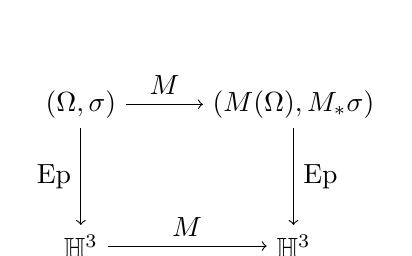
\begin{tikzpicture}[scale=0.9]
\node (1) at (0,2) {$(\Omega,\sigma)$};
\node (2) at (3,2) {$(M(\Omega),M_*\sigma)$};
\node (3) at (0,0) {$\H^3$};
\node (4) at (3,0) {$\H^3$};


\draw[->] (1) to node [above] {$M$} (2);
\draw[->] (1) to node [left] {$\mathrm{Ep}$} (3);
\draw[->] (3) to node [above] {$M$} (4);
\draw[->] (2) to node [right] {$\mathrm{Ep}$} (4);

\end{tikzpicture}
\]
That is, $\mathrm{Ep}_{M_*\sigma}(M(z)) = M( \mathrm{Ep}_{\sigma}(z))$. 
This is because both $M \circ \mathrm{Ep}_\sigma$ and $\mathrm{Ep}_{M_*\sigma} \circ M$ as maps on $\Omega$ satisfy the visual metric condition from Theorem \ref{epstein-map-def} (see \cite{anderson1998} for more details ).

This allows us to define Epstein maps on certain quotients. 
Suppose in general that $\Gamma$ is a subgroup of $\mathrm{SL}_2\C$ acting freely and properly discontinuously on $\H^3 \cup \CP^1$ leaving a domain $\Omega$ invariant. 
Then $\Omega/\Gamma$ inherits a Riemann surface structure. 
Call this structure $X$ and let $\sigma$ be a conformal metric  on $X$.
Lift this to $\tilde{\sigma}$ on $\Omega$, which is $\Gamma$-invariant. 
Then $\mathrm{Ep}_{\tilde{\sigma}}: \Omega \to \H^3$ is $\Gamma$-equivariant and therefore descends to a map $\mathrm{Ep}_\sigma : X \to \H^3/ \Gamma$. 
In particular, when $\Gamma$ is a quasi-Fuchsian group and $\Omega$ a component of the domain of discontinuity, each conformal metric $\sigma$ on the surface at infinity $X$ gives rise to a map from $X$ into the quasi-Fuchsian manifold $M$.

Uniqueness also shows us that the surfaces parallel to an Epstein surface are themselves Epstein surfaces. 
More specifically, let $g^t : U \H^3 \to \H^3$ denote the time-$t$ geodesic flow projected down to $\H^3$.
Thus for a unit tangent vector $v$ on $\H^3$ we have $g^t(v) = \exp_p(tv)$.
Using the lift of an Epstein surface to $U\H^3$ described above, each Epstein surface gives rise to a family of surfaces by applying the geodesic flow (and projecting to $\H^3$). 
That is, we have the flowed surfaces $g^t \circ \widehat{\mathrm{Ep}}_\sigma(\Omega)$. 
These surfaces are themselves Epstein surfaces corresponding to scalar multiples of $\sigma$. 
Indeed, since the parallel flow of a horosphere is a horosphere, we know $[g^t(\widehat{\mathrm{Ep}}_\sigma(z)),z] = [\mathrm{Ep}_\sigma(z),z] + t$. 
This shows us
\[
V_{g^t(\widehat{\mathrm{Ep}}_\sigma(z))}(z) = e^{2[g^t(\widehat{\mathrm{Ep}}_\sigma(z)),z]}\overset{\circ}{\sigma}(z) = e^{2t}e^{2[\mathrm{Ep}_\sigma(z),z]}\overset{\circ}{\sigma}(z) = e^{2t}\sigma(z).
\]
But the unique map that satisfies this equality is $\mathrm{Ep}_{e^{2t}\sigma}$. 
In summary, we have the following lemma, attributed to Thurston (unpublished work) by Epstein in \cite{epstein1984}.
\begin{lem}
\label{epstein-flow}
Let $\Omega$ be a domain in $\CP^1$ and $\sigma$ a conformal metric on $\Omega$.
Then 
\[
g^t \circ \widehat{\mathrm{Ep}}_\sigma  = \mathrm{Ep}_{e^{2t} \sigma}.
\]
That is, flowing the Epstein surface for $\sigma$ for time $t$ in the normal direction corresponds to taking the Epstein surface for the metric $e^{2t}\sigma$.
\end{lem}



%%%%%%%%%%%
\subsection{Geometry of Epstein surfaces}\label{epstein-geometry}
%%%%%%%%%%%



The first fundamental form of the Epstein surface for the metric $\sigma$ is given by $I(\sigma) = \mathrm{Ep}_\sigma^*(g_{\H^3})$ for $g_{\H^3}$ the metric of $\H^3$. 
It is given by 
\[
I(\sigma) = 4|B(g_{\CP^1},\sigma)|^2\sigma^{-1} + \frac{1}{4}(1-K(\sigma))^2\sigma + 2(1-K(\sigma))\text{Re}(B(g_{\CP^1},\sigma)).
\]
The second fundamental form (relative to the normal lift $\widehat{\mathrm{Ep}}_\sigma$) is 
\[
\two(\sigma)
= 4|B(g_{\CP^1},\sigma)|^2\sigma^{-1} - \frac{1}{4} (1 - K(\sigma)^2)\sigma - 2 K(\sigma) \text{Re}(B(g_{\CP^1},\sigma)).
\]
These formulas are derived in \cite[Eqns.~3.2-3.3]{dumas2017}.
Here $K(\sigma)$ is the Gaussian curvature of $\sigma$ and $B(g_{\CP^1},\sigma)$ the Schwarzian derivative of $\sigma$ with respect to a M\"obius flat metric. 
We note that when the Epstein surface is embedded, its second fundamental form is negative definite due to our convenient choice of normal vector field.
Writing $\det(g)$ for the determinant of the matrix representation of $g$ relative to some local frame for the tangent bundle, the metrics on $\sigma$ and $I(\sigma)$ on $S$ have determinants related by
\[
\det(I(\sigma)) = \left( (1-K(\sigma))^2 - 16 |B(g_{\CP^1},\sigma)|^2\sigma^{-2} \right)^2 \det(\sigma).
\]
This equation is independent of the frame and has in intrinsic meaning, namely it describes the ratio of volume forms of these two metrics. 
We can compute the Gaussian curvature by $K(I(\sigma)) = -1 + \det(I(\sigma)^{-1}\two(\sigma))$ and the mean curvature by $H(\mathrm{Ep}_\sigma) = \frac{1}{2}\mathrm{tr}(I(\sigma)^{-1}\two(\sigma))$. 
We obtain
\[
K(I(\sigma))
= \frac{4K(\sigma)}{(1-K(\sigma))^2 - 16|B(g_{\CP^1},\sigma)|^2\sigma^{-2}}
\]
and
\[
H(\mathrm{Ep}_\sigma)
= \frac{K(\sigma)^2 - 1 - 16 |B(g_{\CP^1},\sigma)|^2\sigma^{-2}}{(K(\sigma) - 1)^2 - 16 |B(g_{\CP^1},\sigma)|^2\sigma^{-2}}.
\]

 
In the quasi-Fuchsian setting, if $\sigma$ is a $\Gamma$-invariant conformal metric on $\Omega$ then each term in the above equations is also $\Gamma$-invariant. 
This may be less clear for the quadratic differential $B(g_{\CP^1},\sigma)$ since the M\"obius flat metric $g_{\CP^1}$ is not itself $\Gamma$-invariant. 
However, we see that for $\gamma \in \Gamma$ we have $\gamma^*B(g_{\CP^1},\sigma) = B(\gamma^*g_{\CP^1},\gamma^*\sigma) = B(\gamma^* g_{\CP^1},\sigma)$, by naturality of Schwarzian derivatives of conformal metrics. 
The metric $\gamma^* g_{\CP^1}$ is still a M\"obius flat metric, and so $B(\gamma^* g_{\CP^1},\sigma) = B(g_{\CP^1},\sigma)$, implying $B(g_{\CP^1}, \sigma)$ is $\Gamma$-invariant. 
Therefore, $B(g_{\CP^1},\sigma)$ induces a quadratic differential on $X$, which we will denote by $B(\sigma)$.

In summary of the above, we have the following Gaussian and mean curvatures of the Epstein surfaces in $M$.
\begin{lem}
\label{curvature-epstein}
The Gaussian curvature for the Epstein surface $\mathrm{Ep}_\sigma : X \to M$ is given by
\[
K(I(\sigma))
= \frac{4K(\sigma)}{(1-K(\sigma))^2 - 16 |B(g_{\CP^1},\sigma)|^2\sigma^{-2}},
\]
and the mean curvature by 
\[
\pushQED{\qed}
H(\mathrm{Ep}_\sigma)
= \frac{K(\sigma)^2 - 1 - 16 |B(g_{\CP^1},\sigma)|^2\sigma^{-2}}{(K(\sigma) - 1)^2 - 16 |B(g_{\CP^1},\sigma)|^2\sigma^{-2}}.
\qedhere
\popQED
\]
\end{lem}
These are now equations on the compact Riemann surface $X$.






%%%%%%%%%%%%%%%%%%%%%%%%%%%%%%%%%%%%%%%%%%%%
\section{Asymptotically Poincar\'e Families} \label{main-results-chapter}




Previously, we have discussed Epstein surfaces for domains and for quotients. 
Generalizing this, we say a surface $i : S \to M$ is an Epstein surface of $X$ if there exists a $\Gamma$-invariant conformal metric $\tilde{\sigma}$ on $\Omega$ and a diffeomorphism $\varphi : X \to S$ in the preferred homotopy class (see Section \ref{quasi-fuchsian}) such that the diagram 
\[
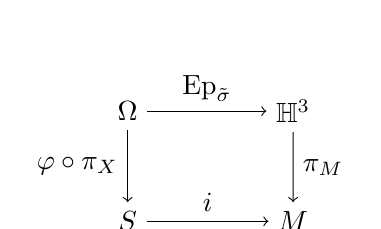
\begin{tikzpicture}[scale=0.7]
\node (1) at (0,2) {$\Omega$};
\node (2) at (3,2) {$\H^3$};
\node (3) at (0,0) {$S$};
\node (4) at (3,0) {$M$};


\draw[->] (1) to node [above] {$\mathrm{Ep}_{\tilde{\sigma}}$} (2);
\draw[->] (1) to node [left] {$\varphi \circ \pi_X$} (3);
\draw[->] (3) to node [above] {$i$} (4);
\draw[->] (2) to node [right] {$\pi_M$} (4);

\end{tikzpicture}
\]
commutes. 
Here the $\pi_X$ and $\pi_M$ are the respective quotient maps $\Omega \to X$ and $\H^3 \to M$.
When $S$ is an Epstein surface of $X$, the conformal metric $\tilde{\sigma}$ induces a conformal metric $\sigma$ on $X$ that we call the conformal metric at infinity. 
We have $\mathrm{Ep}_{\sigma} = \varphi \circ i$. 
The Epstein surface $S$ will then refer to the embedded image of $\mathrm{Ep}_{\sigma}: X \to M$. 

Since $X$ is a closed surface of genus at least 2, it possesses a unique hyperbolic conformal metric $h$. 
Hence, there is a distinguished Epstein surface in $M$. 

\begin{defn}
The Poincar\'e surface of $X$ is the Epstein induced by the Poincar\'e metric of $\Omega$. 
Since the Poincar\'e metric induces the hyperbolic metric $h$ on $X$, the Poincar\'e surface of $X$ is the Epstein surface $\mathrm{Ep}_h: X \to M$.
\end{defn}


Again, we call this a surface but it need not be immersed. 
In fact, we can identify cases when it is not. 
When $\sigma = h$ we know $K(h) = -1$ and $B(h) = \frac{1}{2}\phi$. 
Then using the formula for determinant of $I(h)$ given in Section \ref{epstein-geometry}, we compute
\[
\det(I(h)) = 16 \left( 1 - \frac{|\phi|^2}{h^2} \right)^2 \det(h).
\]
And so we see $\mathrm{Ep}_h$ is not an immersion at points in $X$ where $\frac{|\phi|}{h} =1$. 
However, by parallel flowing of the Poincar\'e surface we eventually obtain an immersed (embedded, actually) surface, which we now discuss. 


The Poincar\'e surface together with its parallel copies forms a family of surfaces we call the Poincar\'e Family. 
Recall from Lemma \ref{epstein-flow} that the parallel copies are given as the Epstein surfaces $\mathrm{Ep}_{e^{2t}h}: X \to M$ for $t \geq 0$. 
This family of surfaces has been a useful tool for studying the geometry of hyperbolic 3-manifolds, see e.g., \cite{anderson1998}, \cite{bromberg2004}, \cite{krasnov-schlenker2008}, and \cite{bridgeman-brock-bromberg2019}.
The surfaces in the Poincar\'e family are eventually embedded as was shown by Anderson \cite{anderson1998} who obtained a specific bound on $t$ that implied embededness. 
We omit the proof here as we will show a more general result in Proposition \ref{asym-family-prop}. 
Although we will show a bound for $t$ after which the Epstein surface for $e^{2t}\sigma$ is immersed. 
Denote by $\|B(\sigma)\|_\sigma$ and $\|K(\sigma)\|$ the supremums over $X$ of the functions $|B(\sigma)|/\sigma$ and $K(\sigma)$, then we have the following.

\begin{lem}\label{parallel-family-immersed}
Let $\sigma$ be a conformal metric on $X$. 
If 
\[
t > \log  \sqrt{ 4 \|B(\sigma)\|_\sigma + \|K(\sigma)\|},
\]
then $\mathrm{Ep}_\sigma: X \to M$ is an immersion.
\end{lem}

\begin{proof}
If $t$ satisfies this bound then we have
\[
e^{2t} > 4 \|B(\sigma)\|_\sigma + \|K(\sigma)\| > 4 \frac{|B(\sigma)|}{\sigma} + K(\sigma)
\]
Rearranging and simplifying, this implies that 
\[
(e^{2t} - K(\sigma))^2 - 16\frac{|B(\sigma)|^2}{\sigma^2} > 0.
\]
It then follows that $\det(I(e^{2t}\sigma)) > 0$ so that $I(e^{2t}\sigma)$ is positive definite. 
\end{proof}

In the Poincar\'e case the this becomes $t > \log \sqrt{2\|\phi\|_h + 1}$, which is the bound obtained by \cite{anderson1998}, although we do not get embeddedness from this lemma. 

So, the Poincar\'e family is the family of Epstein surfaces for the conformal metrics at infinity $\rho_t = e^{2t}h$ and for $t$ sufficiently large these surfaces are embedded. 
We now discuss their asymptotic behavior. 
In order to consider derivatives more easily, let us reparametrize the Poincar\'e family using $\epsilon = e^{-2t}$, so that $\rho_\epsilon = h/\epsilon$. 
We are interested in the behavior as $\epsilon \to 0$. 

Using the formula for the first fundamental form of an Epstein surface we can compute
\[
I(\rho_\epsilon) = \frac{1}{4\epsilon} h + \frac{1}{2} h + \mathrm{Re}(\phi) + \epsilon \left( \frac{1}{4} h + \mathrm{Re}(\phi) + \frac{|\phi|^2}{h} \right).
\]
We can therefore consider the Poincar\'e family as a path in the space of metrics $\mathrm{Met}(S)$. 
The following arguments are formal; they will be made precise in the next section. 
We see the family of first fundamental forms diverges as $\epsilon \to 0$. 
However, rescaling gives
\[
4\epsilon I(\rho_\epsilon) = h + 4\epsilon \left( \frac{1}{2}h + \mathrm{Re}(\phi) \right) + O(\epsilon^2).
\]
And so, if we project to the quotient, we can consider the Poincar\'e family as a path in Teichm\"uller space that converges: $[I(\rho_\epsilon)] \to [h]$ as $\epsilon \to 0$. 
Moreover, differentiating at $0$ yields
\[
\left. \frac{d}{d\epsilon} \right|_{\epsilon = 0} \ 4\epsilon I(\rho_\epsilon) = 2h + 4 \mathrm{Re}(\phi).
\]
Since $2 h $ is pure-trace (with respect to $h$) and since $\mathrm{Re}(\phi)$ is an $h$-transverse-traceless tensor by Lemma \ref{tangent-teich}, we see the tangent vector to this path in Teichm\"uller space at $[h]$ is $\dot{[I(\rho_\epsilon)]} = d \pi_h (2h + 4 \mathrm{Re}(\phi)) = 4 \mathrm{Re}(\phi)$. Similar computations apply to $\two(\rho_\epsilon)$ and show that $[\two(\rho_\epsilon)] \to [h]$ as $\epsilon \to 0$ with tangent vector given by $\dot{[\two(\rho_\epsilon)]} = 0$. 

Summarizing: The Poincar\'e family has the property that the surfaces form a parallel family foliating the end of $M$ such that the paths $[I(\rho_\epsilon)] \to [h]$ and $[\two(\rho_\epsilon)] \to [h]$ in Teichm\"uller space as $\epsilon \to 0$, and $\dot{[I(\rho_\epsilon)]} = 4 \mathrm{Re}(\phi)$ and $\dot{[\two(\rho_\epsilon)]} = 0$. 
It turns out the only thing needed about the the Poincar\'e family to obtain these results is that there is a function $f$ so that $f(\epsilon)\rho_\epsilon \to h$ as $\epsilon \to 0$. 
The function here is the identity $f(\epsilon) = \epsilon$. 
In the next section we introduce a generalization of the Poincar\'e family and discuss the corresponding results that are true for this generalization.



%%%%%%%%%%%
\subsection{Asymptotically Poincar\'e families}
%%%%%%%%%%%
\label{asym-def-section}


The key property of the Poincar\'e family we wish to generalize is that $f(\epsilon)\rho_\epsilon \to h$ for $f(\epsilon) = \epsilon$ as $\epsilon \to 0$. 
We consider, then, families of Epstein surfaces whose conformal metrics at infinity $\sigma(\epsilon)$ satisfy $f(\epsilon)\sigma(\epsilon) \to h$ as $\epsilon \to 0$ where now $f$ is any positive smooth function with the same behavior to first order at $0$, i.e., that $f(0) = 0$, and $f'(0) \neq 0$. 
As we will soon make arguments regarding the regularity of the tensors we consider, we will add regularity designations to our spaces, e.g., the space of smooth metrics on $X$ will be denoted by $\mathrm{Met}^\infty(X)$ and the space of smooth conformal metics will be $\mathrm{Conf}^\infty(X)$.



\begin{defn}
\label{asym-def}
Let $S_\epsilon$ for $\epsilon$ in $(0,1)$ be a family of embedded Epstein surfaces with conformal metrics at infinity $\sigma(\epsilon)$. 
We call this family \textit{asymptotically Poincar\'e} if 
\begin{enumerate}
    \item there exists a scaling function $f:[0,1) \to [0,\infty)$ so that the path 
    \[
f\sigma:(0,1) \to \mathrm{Met}^\infty(X)
\]
is differentiable and converges to the hyperbolic metric on $X$ as $\epsilon \to 0$, that is, $f(\epsilon)\sigma(\epsilon) \to h$ as $\epsilon \to 0$,
    \item the function $f$ is smooth and has simple zero at 0, and
    \item the continuous extension $\gamma:[0,1) \to \mathrm{Met}^\infty(X)$ of $f \sigma$ is differentiable.
\end{enumerate}

\end{defn}


The surfaces in the Poincar\'e family are parallel to one another. The surfaces in an asymptotically Poincar\'e family are asymptotically parallel in the sense of the following lemma. 
 




\begin{lem}\label{asym-parallel-lemma}
Suppose $S_\epsilon$ is an asymptotically Poincar\'e family of surfaces. 
Let $t > 0$. 
If $g^t$ is the geodesic flow operator defined above, then  
\[
d_M \left(g^t (\widehat{\mathrm{Ep}}_{\sigma(\epsilon)}(z)), \mathrm{Ep}_{\sigma(e^{-2t} \epsilon)}(z) \right) \to 0
\quad \text{ as } \epsilon \to 0
\]
uniformly in $z$. 
That is, the distance between the surface $S_\epsilon$ flowed for time $t$ and the surface $S_{e^{-2t}\epsilon}$ tends towards zero as $\epsilon$ does. 
\end{lem}


\begin{proof}
We work with the universal covers. 
In general, a straightforward computation using the $\mathrm{SL}_2\C$-frame definition of the Epstein  map $\Omega \to \H^3$ gives the distance between the image of $z$ under the Epstein map for the metrics $\sigma = e^{2\eta}|dz|^2$ and $\tau =e^{2\lambda}|dz|^2$ as
\begin{align*}
d_{\H^3} \left( \mathrm{Ep}_{\sigma}(z), \mathrm{Ep}_{\tau}(z) \right)
&= 2 \mathrm{arctanh} \left(\sqrt{ \frac{(e^\eta - e^{\lambda})^2  + 4|\eta_z - \lambda_z|^2}{(e^\eta + e^{\lambda})^2  + 4|\eta_z - \lambda_z|^2}} \right)
\end{align*}
where all functions are evaluated at $z$, which we have suppressed for brevity.

In our case, lift $\sigma(\epsilon)$ to $\tilde{\sigma}(\epsilon)$ and $\gamma(\epsilon) = f(\epsilon)\sigma(\epsilon)$ to $\tilde{\gamma}(\epsilon)$ on $\Omega$. 
Write $\tilde{\sigma}(\epsilon) = e^{2\eta(\epsilon)}|dz|^2$ and $\tilde{\gamma}(\epsilon) = e^{2\lambda(\epsilon)}|dz|^2$, then $\eta(\epsilon) = \lambda(\epsilon) - (1/2)\log(f(\epsilon))$. 
Recall from Lemma \ref{epstein-flow} that $g^t \circ \widehat{\mathrm{Ep}}_{\tilde{\sigma}(\epsilon)} = \mathrm{Ep}_{e^{2t}\tilde{\sigma}(\epsilon)}$.
For ease of notation, let $c = e^{-2t}$. 
Then we have the distance between $\mathrm{Ep}_{c^{-1} \tilde{\sigma}(\epsilon)}$ and $\mathrm{Ep}_{\tilde{\sigma}(c\epsilon)}$ can be simplified to
\[
2 \mathrm{arctanh} \left(\sqrt{ 
\frac
{(1 - \sqrt{\frac{c f(\epsilon)}{f(c \epsilon)}}e^{\lambda(c\epsilon) - \lambda(\epsilon)})^2 + 4 c f(\epsilon)e^{-2\lambda(\epsilon)}|\lambda_z(c\epsilon) - \lambda_z(\epsilon)|^2}
{(1 + \sqrt{\frac{c f(\epsilon)}{f(c \epsilon)}}e^{\lambda(c\epsilon) - \lambda(\epsilon)})^2 + 4 c f(\epsilon)e^{-2\lambda(\epsilon)}|\lambda_z(c\epsilon) - \lambda_z(\epsilon)|^2}
} \right).
\] 
Since $\tilde{\gamma}(\epsilon)$ converges in $\mathrm{Met}^\infty(X)$, the function $\lambda$ has a $C^2$ limit as $\epsilon \to 0$. 
Therefore, the argument of $\mathrm{arctanh}$ converges to zero uniformly in $z$.

Since the distance between the surfaces in the universal cover is converging to zero, and since the quotient map $\H^3 \to M$ is a local isometry, we get the Lemma. 
\end{proof}



We have required that an asymptotically Poincar\'e family consist of embedded surfaces.
The next proposition gives a useful condition for a family of conformal metrics to give rise to an asymptotically Poincar\'e family of surfaces. 




\begin{prop}
\label{asym-family-prop}
Let $\sigma: (0,1) \to \mathrm{Conf}^\infty(X)$ be a family of conformal metrics on $X$. 
Suppose there exists a smooth function $f:[0,1) \to [0,\infty)$ with simple zero at $0$, such that $f\sigma \to h$ as $\epsilon \to 0$ and such that the extension $\gamma: [0,1) \to \mathrm{Conf}^\infty(X)$ is differentiable.
Then there exists an $\epsilon_0 >0$ so that for $\epsilon < \epsilon_0$, the Epstein map $\mathrm{Ep}_{\sigma(\epsilon)}$ is an embedding. 
Hence, the Epstein surfaces $\mathrm{Ep}_{\sigma(\epsilon)}:X \to M$, for $\epsilon < \epsilon_0$, form an asymptotically Poincar\'e family. 
\end{prop}

\begin{proof} 
Let $\tilde{\sigma}:(0,1) \to \mathrm{Conf}^\infty(\Omega)$ be the lift of the family $\sigma$. 
Define the Epstein family map $\mathrm{Ep}_{\tilde{\sigma}}: \Omega \times (0,1) \to \H^3$ by $\mathrm{Ep}_{\tilde{\sigma}}(z,\epsilon) = \mathrm{Ep}_{\tilde{\sigma}(\epsilon)}(z)$. 
It follows from the $\mathrm{SL}_2\C$-frame definition of the Epstein map that in the upper half space model $\H^3 \cong \C \times \R^+$, the family map is given by 
\[
\mathrm{Ep}_{\tilde{\sigma}}(z,\epsilon) = (z,0) + \frac{2}{e^{2\eta} + 4 |\eta_z|^2}\left(2 \eta_{\bar{z}}, e^\eta \right).
\]
Writing $\tilde{\sigma}(\epsilon) = e^{2 \eta(z,\epsilon)}|dz|^2$ and $\tilde{\gamma}(\epsilon) = e^{2 \lambda(z,\epsilon)}|dz|^2$, the condition $\tilde{\gamma}(\epsilon) = f(\epsilon)\tilde{\sigma}(\epsilon)$ becomes $\eta(z,\epsilon) = \lambda(z,\epsilon) - (1/2) \log(f(\epsilon))$.
Note that $\lambda(z,\epsilon) \to \rho(z)$ as $\epsilon \to 0$, uniformly in $z$, where $\rho$ is the log density of the Poincar\'e metric of $\Omega$. 
Hence we can rewrite $\mathrm{Ep}_{\tilde{\sigma}}$ as 
\[
\mathrm{Ep}_{\tilde{\sigma}}(z,\epsilon) = (z,0)  + \frac{2}{e^{2\lambda} + 4 f(\epsilon) |\lambda_z|^2} \left( 2 f(\epsilon) \lambda_{\bar{z}},  \sqrt{f(\epsilon)}e^{\lambda} \right)
\]
and see that
\[
\lim_{\epsilon \to 0} \mathrm{Ep}_{\tilde{\sigma}} (z,\epsilon) = (z,0).
\]
So we may extend $\mathrm{Ep}_{\tilde{\sigma}}$ to a map $\Omega \times [0,1) \to \H^3 \sqcup \Omega$, which is the identity on the boundary $\Omega \times \{0\} \to \Omega$. 

While this map is not differentiable at $\epsilon = 0$ (due to the $\sqrt{f(\epsilon)}$), the map $F: \Omega \times [0,1) \to \H^3 \sqcup \Omega$ given by $F(z,\epsilon) = \mathrm{Ep}_{\tilde{\sigma}}(z,\epsilon^2)$ satisfies $F(z,0) = (z,0)$, is differentiable at $\epsilon = 0$, and has derivative  
\[
d F_{(z,0)} = 
\begin{pmatrix}
1 & 0 & 0 \\
0 & 1 & 0 \\
0 & 0 & 2 \sqrt{f'(0)} e^{-\rho(z)}
\end{pmatrix}.
\]
Since this is invertible, $F$ is a local $C^1$-diffeomorphism at the boundary of $\Omega \times [0,1) \to \H^3 \sqcup \Omega$.

Define $\bar{M} = ( \H^3 \sqcup \Omega ) /\Gamma = M \sqcup X$.
Then $\bar{M}$ is a smooth manifold with compact boundary $X$. 
By $\Gamma$-equivariance of $\mathrm{Ep}_{\tilde{\sigma}}$, $F$ descends to a map $X \times[0,1) \to \bar{M}$ that is the identity on the boundary $\partial(X \times [0,1)) \to \partial{\bar{M}} = X$ and that is a local diffeomorphism there. 
We now show this implies the restriction of $F$ to $X \times [0, \delta)$, for some small enough $\delta$, is a diffeomorphism onto a collar neighborhood of $\partial \bar{M} = X$. 

Given $(z,0)$ there exists neighborhoods $U_{(z,0)}$ and $V_{(z,0)}$ such that $F: U_{(z,0)} \to V_{(z,0)}$ is a diffeomorphism. 
By compactness of $X$ we may take a finite number $U_i$ and $V_i$ such that $X \times \{0\} \subset \cup U_i$. Call $\cup_i U_i = U$ and $\cup_i V_i = V$. Then $F: U \to V$ is a local diffeomorphism and $X \times \{0\} \subset U, V$. 
In fact, we have 
\begin{lem*}
There exists $\epsilon,\delta > 0$ such that $X \times [0,\delta] \subset U$, and $X \times [0,\epsilon] \subset V$ and such that $X \times [0,\epsilon) \subset F(X \times [0,\delta))$.
\end{lem*}
\begin{proof}
By construction of $U$ there exists a $\delta'$ such that $X \times [0,\delta') \subset U$. So choose $\delta = \delta'/2$. Then $X \times [0, \delta] \subset U$.
We show that there is an $\epsilon > 0$ so that $X \times [0,\epsilon) \subset F(X \times [0,\delta))$, as if this is true, we may replace $\epsilon$ with $\epsilon/2$ to get $X \times [0,\epsilon] \subset V$.

Now, suppose no such $\epsilon$ exists. 
Take a sequence $\epsilon_n \to 0$. 
Then for each $n$ there exists $(w_n, t_n) \in X \times [0, \epsilon_n)$ such that $(w_n,t_n) \notin F(X \times [0,\delta))$. 
But $t_n < \epsilon_n \to 0$. 
Moreover, by compactness of $X$ there exists a subsequence (which we still call) $w_n$ that converges to, say, $w \in X$. 
Then $(w_n,t_n) \to (w,0)$. 
Since $F$ is a local diffeomorphism, there is a neighborhood $W$ of $(w,0)$, which we may assume is a subset of $X \times [0,\delta)$ by taking intersections if needed, that is diffeomorphic to a neighborhood $F(W)$ of $(w,0)$. 
Since $(w_n, t_n) \to (w,0)$, for large enough $n$ we get $(w_n,t_n) \in F(W) \subset F(X \times [0,\delta))$. 
This is a contradiction. 
Hence, we get an $\epsilon >0$ so that $X \times [0,\epsilon) \subset F(X \times [0,\delta))$.
\end{proof}

\begin{cor*}
$X \times [0,\epsilon] \subset F(X \times [0,\delta])$
\end{cor*}

\begin{lem*}
$F: X \times [0,\delta] \to F(X \times [0,\delta])$ is a covering. 
\end{lem*}

\begin{proof}
$F$ is a local diffeomorphism since $X \times [0,\delta] \subset U$ and $X \times [0,\epsilon] \subset V$ and since $F: U \to V$ is a local diffeomorphism. 
Since $X \times [0,\delta]$ is compact, $F$ is a proper mapping and proper local diffeomorphisms are coverings. 
\end{proof}

\begin{lem*}
The covering is trivial. 
\end{lem*}

\begin{proof}
Note that the cardinality of the fibers of $F: X \times [0,\delta] \to F(X \times [0,\delta])$ are constant since everything is connected. 
Also note that $F( X \times (0,\delta]) \subset X \times (0,1)$ and $F: X \times \{0\} \to X \times \{0\}$ is the identity, implying $F^{-1}(\{(w,0)\}) = \{(w,0)\}$. 
Hence, $F: X \times [0,\delta] \to F(X \times [0,\delta])$ is injective. 
\end{proof}

\begin{cor*}
$F: X \times [0,\delta] \to F(X \times [0,\delta])$ is injective and contains a neighborhood of $X \times \{0\}$.
\end{cor*}



Unraveling, we get that $\mathrm{Ep}_{\sigma}$ is a diffeomorphism from a collar neighborhood $X \times (0,\sqrt{\delta})$ to a neighborhood of infinity of $M$.
In particular, each Epstein surface $\mathrm{Ep}_\sigma(\cdot, \epsilon) = \mathrm{Ep}_{\sigma(\epsilon)}$, for $\epsilon < \sqrt{\delta}$, is an immersion and injective with compact domain $X$. 
Hence each Epstein surface, for $\epsilon < \sqrt{\delta}$, is embedded.
To complete the proof take $\epsilon_0 = \sqrt{\delta}$.

\end{proof}


The Poincar\'e family foliates the end of $M$ since they are parallel. 
In the preceding proof, we have the map $F: X \times [0,\delta) \to \bar{M}$ is a diffeomorphism onto its image. 
Hence we have the following result for asymptotically Poincar\'e families.

\begin{cor}
\label{foliation}
If $S_\epsilon$ is an asymptotically Poincar\'e family of surfaces, then there exists an $\epsilon_0 > 0$ such that for $\epsilon < \epsilon_0$ the surfaces $S_\epsilon$ form a foliation of the end of $M$ whose surface at infinity is $X$.
\qed
\end{cor}



We soon turn to our main result, but first recall that the co-orientation on an Epstein surface we are using is that induced by the lift $\widehat{\mathrm{Ep}}_\sigma$, which points towards the surface at infinity $X$.
This implies that $\two(\sigma)$ is negative definite (for small enough $\epsilon$), and so $-\two(\sigma)$ is a smooth Riemannian metric. 
Also recall we are using the Riemannian model of Teichm\"uller space. 
That is, we use 
\[
\mathcal{T}(X) = \mathrm{Met}^\infty(X)/  \left( \mathrm{Diff}_0^\infty(X) \ltimes P^\infty(X) \right),
\]
where $P^\infty(X)$ is the set of smooth positive functions on $X$ and $\mathrm{Diff}_0^\infty(X)$ is the group of smooth diffeomorphisms isotopic to the identity (see \cite{tromba1992} for details). 
The smooth topology, however, is difficult to work with directly. 
So, we work in the Sobolev setting for tensors and functions.



%%%%%%%%%%%
\subsection{Sobolev spaces on manifolds} \label{sobolev}
%%%%%%%%%%%

The Sobolev setting is useful because they form Banach spaces, which enjoy the standard tools of analysis. Most notably, the familiar inverse and implicit function theorem are available in this setting.  

To define the relevant Sobolev spaces on the closed surface $S$ we need to fix a background Riemannian metric, the natural choice being the hyperbolic metric $h$. 
Let $\nabla$ be its Levi-Civita connection. 
Both $h$ and $\nabla$ extend to metrics and connections on all the tensor bundles on $S$ made from $TS$ and $T^*S$. 
Hence all tensor bundles have a norm induced by $h$. 
Let $\mathscr{T}^{(k,l)}(S)$ be the space of smooth $(k,l)$-tensor fields on $S$. 
The space $W^{s,p}(\mathscr{T}^{(k,l)}(S))$ will denote the space of Sobolev tensors. 
It is the completion of $\mathscr{T}^{(k,l)}(S)$ under the norm
\[
\|T\|_{s,p} = \left( \sum_{j = 0}^s \int_S | \nabla^j T|^p \ dVol(h) \right)^{1/p}.
\]
Here $\nabla^j$ is the iterated covariant derivative ($j$-times). 

Compactness of $S$ is vital here as it guarantees this norm is finite. 
These Sobolev spaces are Banach spaces and when $p = 2$ they are Hilbert spaces. 
We will denote them by $H^s(\mathscr{T}^{(k,l)}(S))$ (note: this is not cohomology). 
The spaces in which we will be most interested are the Sobolev spaces of real-valued functions $H^s(S,\R)$, metrics $\mathrm{Met}^s(S)$, and conformal metrics $\mathrm{Conf}^s(X)$.

Sobolev functions (or tensors) that satisfy an equation in the sense of distributions are called weak solutions to the equation. 
On $S$, where the dimension is 2, the Sobolev Embedding Theorem on smooth surfaces guarantees that weak solutions in $H^s$ for $s \geq 3$ are actually strong solutions, being $C^{2,\alpha}$-regular \cite{aubin1982}. 
We will therefore assume $s \geq 3$ from now on. 
We also note that $C^\infty = \cap_s H^s$.


In this Sobolev setting the space of symmetric 2-tensors is a Hilbert space. Hence, the tangent space to $\mathrm{Met}^s(X)$ at $g$ may is a be decomposed as the orthogonal sum
\[
T_g \mathrm{Met}^s(X) = \{\dot{g} \ | \ \mathrm{tr}_g (\dot{g}) = 0 = \mathrm{div}_g(\dot{g}) \} \oplus \{\mathcal{L}_X g + fg \ |\ f \in H^s \text{ and } X \in \Gamma(TX) \},
\] 
where $\mathrm{div}_g(\dot{g})$ is the divergence of the 1-1 tensor $g^{-1}\dot{g}$. 
The second summand is tangent to the $\mathrm{Diff}_0^s(X) \rtimes P^s(X)$ orbit of $g$ and the first summand is the transverse traceless tensors consisting of elements that are smooth, trace-free, and divergence-free (see \cite{fischer-marsden1975} for more details). 
Since the transverse traceless tensors are orthogonal to the group orbit they may be identified with the tangent space $T_{[g]} \left( \mathrm{Met}^s(X)/ \mathrm{Diff}_0^s(X) \rtimes P^s(X) \right)$ to the quotient at $[g]$. 
Moreover transverse traceless tensors are a set of smooth tensors that are $L^2$ orthogonal to the $\mathrm{Diff}_0^s(X) \rtimes P^s(X)$ orbit \textit{for any} $s$. 
Consequently, they may be identified with the tangent space to the quotient $\mathrm{Met}^\infty(X)/(\mathrm{Diff}_0^\infty(X) \rtimes P^\infty(X))$. 
That is, they may be naturally identified with the tangent space to Teichm\"uller space at $[g]$:
\[
T_{[g]} \mathcal{T}(X) = \{\dot{g} \ | \ \mathrm{tr}_g (\dot{g}) = 0 = \mathrm{div}_g(\dot{g}) \}.
\]
Under this identification, the action of the derivative of the projection $\pi: \mathrm{Met}^\infty(X) \to \mathcal{T}(X)$ at $g$ is given by orthogonal projection onto the transverse traceless tensors $T_g \mathrm{Met}^\infty(X) \to \{\dot{g} \ | \ \mathrm{tr}_g (\dot{g}) = 0 = \mathrm{div}_g(\dot{g}) \}$.



%%%%%%%%%%%
\subsection{Main results}
%%%%%%%%%%%



So, we work in the Sobolev setting of functions $H^s(X)$ and tensors $\mathrm{Met}^s(X)$ and $\mathrm{Conf}^s(X)$.
Since $K$ and $B$ are smooth functions of $\sigma$ and its derivatives we have that they both extend to functions on Sobolev classes of metrics.
Hence if $\sigma \in \mathrm{Conf}^s(X)$ then $I(\sigma)$ and $-\two(\sigma)$ belongs to $\mathrm{Met}^{s-2}(X)$.
We will obtain results with these extensions and then argue our results are independent of the chosen $s$. 



\begin{prop}
\label{thm-in-sobolev}
Suppose $S_\epsilon$ is an asymptotically Poincar\'e family of surfaces. 
Let $\gamma : [0,1) \to \mathrm{Met}^s(X)$ be the extension of $f\sigma$ thought of as taking values in a class of Sobolev metrics for a fixed $s > 3$. 
Then the first and second fundamental forms $I \circ \sigma: (0,1) \to \mathrm{Met}^{s-2}(X)$ and  $\two \circ \sigma: (0,1) \to \mathrm{Met}^{s-2}(X)$ satisfy
\[
I_\epsilon := 4 f'(0) \epsilon I(\sigma(\epsilon)) \to h
\quad \text{ and } \quad
\two_\epsilon :=  - 4 f'(0) \epsilon \two(\sigma(\epsilon)) \to h
\quad \text{ as } \epsilon \to 0.
\]
Moreover, $I_\epsilon$ and $\two_\epsilon$ are differentiable at $\epsilon = 0$ and their tangent vectors are given by 
\[
\dot{I_\epsilon} = \dot{\gamma} + 2 f'(0) h + 4 f'(0) \mathrm{Re}(\phi)
\quad \text{ and } \quad
\dot{\two_\epsilon} = \dot{\gamma}
\]
\end{prop}

\begin{proof}
We have that $\gamma:[0,1) \to \mathrm{Met}^\infty(X)$ is continuous and differentiable at $\epsilon = 0$. 
Therefore, as $\mathrm{Met}^\infty(X) = \cap_{s > 3} \mathrm{Met}^s(X)$ we also have that $\gamma$ is continuous to $\mathrm{Met}^s$ and differentiable at $\epsilon = 0$. 

Then, we have $I(\sigma(\epsilon)) = I(\frac{1}{f(\epsilon)} \gamma(\epsilon))$ is equal to 
\[
4 f(\epsilon) \frac{|B(\gamma(\epsilon))|^2}{\gamma(\epsilon)} + \frac{1}{4 f(\epsilon)}(1 - f(\epsilon) K(\gamma(\epsilon)))^2 \gamma(\epsilon) + 2(1 - f(\epsilon)K(\gamma(\epsilon)))\mathrm{Re}(B(\gamma(\epsilon))),
\]
which is a smooth tensor independent of $s$. 
Since $f:[0,1) \to \R$ and $\gamma:[0,1) \to \mathrm{Met}^s(X)$ are differentiable at 0 and since $K: \mathrm{Met}^s(X) \to H^{s-2}(X)$ and $B: \mathrm{Conf}^s(X) \to \Gamma^{s-2}(\Sigma^{2}(X))$ are differentiable at the hyperbolic metric $h$, we can write 
\begin{align*}
f(\epsilon) = \epsilon f'(0) + O(\epsilon^2), \quad
K(\gamma(\epsilon)) = -1 + O(\epsilon), \quad 
B(\gamma(\epsilon)) = \frac{1}{2} \phi + O(\epsilon).
\end{align*}

Substitution and some simplification gives 
\[
I(\sigma(\epsilon)) = \frac{1}{4\epsilon f'(0)} h + \frac{1}{4 f'(0)} \dot{\gamma} + \frac{1}{2} h + \mathrm{Re}(\phi) + O(\epsilon).
\]
Consequently, 
\[
I_\epsilon =  h + \epsilon(\dot{\gamma} + 2 f'(0)h + 4 f'(0) \mathrm{Re}(\phi)) + O(\epsilon^2).
\]
The same reasoning will give 
\[
\two_\epsilon = h + \epsilon \dot{\gamma} + O(\epsilon^2).
\]
The result then follows.
\end{proof}


We now prove our main result, Theorem \ref{main-thm-intro} from the Introduction. 
Recall that $[\two]$ denotes the point in Teichm\"uller space corresponding to the conformal class of $-\two$.


\begin{thm}\label{main-result}
Let $S_\epsilon$ for $\epsilon \in (0,1)$ be an asymptotically Poincar\'e family of surfaces with metrics at infinity $\sigma(\epsilon)$. 
If $h$ is the hyperbolic metric of $X$ and $\phi$  the holomorphic quadratic differential at infinity, then in Teichm\"uller space $\mathcal{T}(X)$ we have 
\[
[I(\sigma(\epsilon))] \to [h]
\quad \text{ and } \quad
[\two(\sigma(\epsilon))] \to [h]
\quad \text{ as } \epsilon \to 0.
\]
Moreover, the tangent vectors in $T_{[h]} \mathcal{T}(X)$ are given by 
\[
\dot{[I(\sigma(\epsilon))]}  = 4 f'(0) \mathrm{Re}(\phi) \quad \text{ and } \quad \dot{[\two(\sigma(\epsilon))]} = 0.
\]
\end{thm}

\begin{proof}
Using the notation from  Proposition \ref{thm-in-sobolev}, for each $s > 3$ we have that $I_\epsilon$ and $\two_\epsilon$, which are paths through smooth tensors, converge in $\mathrm{Met}^s(X)$ to the hyperbolic metric $h$. 
Since $\mathrm{Met}^\infty(X)  = \cap \mathrm{Met}^s(X)$ we know that $I_\epsilon$ and $\two_\epsilon$ converge to $h$ in $\mathrm{Met}^\infty(X)$. 
Moreover, since the projection $\mathrm{Met}^\infty(X) \to \mathcal{T}(X)$ is continuous, and since $[I(\sigma(\epsilon))] = [I_\epsilon]$ and $[\two(\sigma(\epsilon))] = [\two_\epsilon]$, we have that
\[
[I(\sigma(\epsilon))] \to [h]
\quad \text{ and } \quad 
[\two(\sigma(\epsilon))] \to [h]
\quad \text{ as } \epsilon \to 0.
\]
Since both paths converge to $[h]$ at $\epsilon = 0$ we can extend them to continuous paths $[0,1) \to \mathcal{T}(S)$. 
Since $[I(\sigma(\epsilon))]$ and  $[\two(\sigma(\epsilon))]$ agree with $[I_\epsilon]$ and $[\two_\epsilon]$, respectively, we also have they are differentiable at $\epsilon = 0$.

From Proposition \ref{thm-in-sobolev} we know that 
\[
\dot{I_\epsilon}  = \dot{\gamma} + 2 f'(0) h + 4 f'(0) \mathrm{Re}(\phi) \quad \text{ and } \quad \dot{\two_\epsilon} = \dot{\gamma}.
\]
Since $\phi$ is holomorphic, $4 f'(0) \mathrm{Re}(\phi)$ is trace-free and divergence-free. 
On the other hand, $2 f'(0) h$ is pure trace and so belongs to the $\mathrm{Diff}_0^s(X) \rtimes P^s(X)$ orbit of $h$. Furthermore, for any $s$ it belongs to the group orbit of $h$. 
Hence, the derivative of the projection at $h$ removes this term.
Similarly, $\gamma$ is a path in the group orbit of $h$ and so $\dot{\gamma}$ projects to 0. 
We then have
\begin{align*}
\dot{[I(\sigma(\epsilon))]}
= \dot{[I_\epsilon]}
= d \pi_h (\dot{\gamma} + 2 f'(0) h + 4 f'(0) \mathrm{Re}(\phi)) 
= 4 f'(0) \mathrm{Re}(\phi)
\end{align*}
and
\[
\dot{[\two(\sigma(\epsilon))]} = \dot{\two_\epsilon} = d \pi_h (\dot{\gamma}) = 0,
\]
as claimed.
\end{proof}


%%%%%%%%%%%%%%%%%%%%%%%%%%%%
\section{Applications of Asymptotically Poincar\'e Families} \label{applications}




In this section we discuss some applications of Theorem \ref{main-result}. 



%%%%%%%%%%%
\subsection{A conjecture of Labourie}
%%%%%%%%%%%



Labourie proved in \cite{labourie1991} that geometrically finite ends of hyperbolic 3-manifolds admit foliations by surfaces of constant Gaussian curvature. 
These he called $k$-surfaces and for each $k \in (-1,0)$ there exists a unique surface in the foliation whose curvature is identically $k$.
Both ends of a quasi-Fuchsian manifold are geometrically finite, hence this foliation result applies in the quasi-Fuchsian case.

Focusing on one end of the quasi-Fuchsian manifold with surface at infinity $X$, in \cite{labourie1992} Labourie discusses how the conformal classes $[I_k]$ and $[\two_k]$ of the first and second fundamental forms of the $k$-surfaces behave as paths in the Teichm\"uller space of $X$. 
When $k \to -1$, he proves that $[\two_k]$ approaches the point at infinity of $\mathcal{T}(X)$ corresponding to the measured geodesic lamination on the convex core of the quasi-Fuchsian manifold. 
When $k \to 0$, he showed both $[I_k]$ and $[\two_k]$ converge to the same point: the complex structure $X$ on the surface at infinity; or in metric terms, converge to the class of the hyperbolic metric $[h]$.
He conjectures that the tangent vector to these paths is related to the holomorphic quadratic differential at infinity $\phi$. 

We establish his conjecture later in this chapter (Theorem \ref{labourie-conjecture-proof}). 
Indeed, Labourie's $k$-surfaces form an asymptotically Poincar\'e family (as we will show). 
Therefore, our main result Theorem \ref{main-result} applies, describing the asymptotic behavior of the $k$-surfaces as $k \to 0$. 
In the process, our work gives an alternative proof to Labourie's theorem on the existence of $k$-surfaces (at least for $k$ near 0), in this case for quasi-Fuchsian manifolds: see Theorem \ref{k-surfaces-existence}.



%%%%%%%%%%%
\subsection{The $k$-surface equation}
%%%%%%%%%%%



We now prove that $k$-surfaces form an asymptotically Poincar\'e family of surfaces. 
To do this we derive an equation for a conformal metric that implies its Epstein surface is a $k$-surface and we show this equation has a unique smooth solution for each $k$ near zero. 
In the proof of existence of solutions we will see that these conformal metrics satisfy the hypothesis of Proposition \ref{asym-family-prop}. 



Finding a metric $\sigma$ whose Epstein surface has constant Gaussian curvature $k$ is finding a metric $\sigma$ that solves $K(I(\sigma)) = k$, which from Lemma \ref{curvature-epstein} is solving
\[
\frac{4K(\sigma)}{(1-K(\sigma))^2 - 16|B(\sigma)|^2\sigma^{-2}} = k.
\]
For now we will focus on solving
\begin{equation}
\label{k-surface-equation}
4K(\sigma) = k \left((1-K(\sigma))^2 - 16|B(\sigma)|^2\sigma^{-2} \right),
\end{equation}
as we will see that for small enough $k$, $K(I(\sigma)) = k$.

We are interested in obtaining solutions to (\ref{k-surface-equation}) for $k$ near zero. 
This is hampered by the fact that there are no solutions to (\ref{k-surface-equation}) when $k = 0$. 
Indeed we would be asking for $K(\sigma)=0$, which is impossible on a surface with genus bigger than 1. 
In an attempt to obtain better asymptotics we consider the case when $\Gamma$ is Fuchsian. 
Here we have explicit solutions to the $k$-surface equation (\ref{k-surface-equation}).
Indeed, the $k$-surfaces are the Poincar\'e family. 
Working in the universal covers, $\mathrm{Ep}_h : \Omega \to \H^3$ gives a totally geodesic copy of $\H^2$ in $\H^3$ with constant curvature $-1$. 
For $-1<k<0$  the $k$-surfaces are given by equidistant copies of this $\H^2$. 
The conformal metric whose Epstein surface is the $k$-surface is then $c(k)h$ for some function of $k$ satisfying $K(I(c(k)h)) = k$. 
Since $B(g_{\CP^1},c(k)h) = 0$ we get the defining equation of $c$ as $4K(c(k)h) = k(1 - K(c(k)h))^2$.
More explicitly $c$ is given by
\[
c(k) = \frac{1+\sqrt{1+k}}{1-\sqrt{1+k}}.
\]


Suppose we have solution metrics $\sigma_k$  on $X$ that give Epstein surfaces with constant Gaussian curvature $k$. 
As we just saw, in the Fuchsian case we have $\sigma_k = c(k) h$.  
In the general quasi-Fuchsian case, define $f(k)$ by 
\[
f(k) = c(k)^{-1} = \frac{1-\sqrt{1+k}}{1+\sqrt{1+k}}
\] 
and $\tau_k$ by $\tau_k = f(k)\sigma_k$, so that in the Fuchsian case the metric $\tau_k$ is the hyperbolic metric for all $k$. 
Since $\sigma_k$ solves (\ref{k-surface-equation}), by substitution and some simplification we get that $\tau = \tau_k$ solves the equation 
\begin{equation}
\label{scaled-equation}
(2+k)(1+K(\tau))^2 + 2\sqrt{1+k}\left(1-K(\tau)^2\right) + 16\left(2\sqrt{1+k} - 2 - k  \right)\frac{|B(\tau)|^2}{\tau^2} = 0.
\end{equation}


In the limiting case $k=0$ we see that the hyperbolic metric $h$ on $X$ solves (\ref{scaled-equation}). 
Solutions actually exists in a neighborhood of $(k,\tau) = (0,h)$ as we will show.
To apply PDE theory we define the function $F : U \times \mathrm{Conf}^\infty(X) \to C^\infty(X)$ given by 
\[
F(k,\tau) = (2+k)(1+K(\tau))^2 + 2\sqrt{1+k}\left(1-K(\tau)^2 \right) +16\left(2\sqrt{1+k} - 2 - k  \right)\frac{|B(\tau)|^2}{\tau^2}.
\]
Here, $U$ is an open interval around $0$ small enough not to contain $-1$ so that $F$ is smooth on its domain. 
Points $(k,\tau)$ where $F(k,\tau) = 0$ are solutions to the scaled equation (\ref{scaled-equation}); we have already found $F(0,h) = 0$.
 
 
 
%%%%%%%%%%%
\subsection{Solutions to the $k$-surface equation} 
%%%%%%%%%%%



We will use the Implicit Function Theorem in the Banach space setting to obtain solutions to $F(k,\tau) = 0$ and so we first work with $\mathrm{Conf}^s(X) = \{ p h \ |\ p \in H^s(X,\R^+)\}$, where $H^s(X,\R^+)$ is the Sobolev space of functions on $X$ taking positive values.
With the norm $\|\tau\|_s := \| \tau/h\|_s$, the set $\mathrm{Conf}^s(X)$ is naturally identified with an open subset of the Banach space $H^s(X) = H^{s}(X,\R)$.
As stated above, we work with Sobolev spaces of a fixed regularity $s > 3$.
Recall the function $F$ is defined on $U \times \mathrm{Conf}^\infty(X)$ and maps to $C^\infty(X)$. 
Extend $F$ to a function $U \times \mathrm{Conf}^s(X) \to H^{s-2}(X)$ so that $F$ is then defined on an open subset of a Banach space. 

We still have $F(0,h) = 0$ and we can now get solutions near $0$ as well.



\begin{thm}
\label{weak-solutions}
There is a neighborhood $V$ of $0$ such that for each $k \in V$, there exists a unique $\tau \in \mathrm{Conf}^s(X)$ such that $F(k,\tau) = 0$.
\end{thm}

\begin{proof} 
Note that since the constituent parts of $F$ are smooth on $U$, $F$ is smooth. 
Furthermore, $D_2F_{(0,h)} : H^s(X) \to H^{s-2}(X)$ is an isomorphism, where $D_2F$ is the partial derivative of $F$ with respect to its second argument. 
Indeed, a direct computation of the derivative of $F$ at $(0,h)$ yields 
\[
DF_{(0,h)}(\dot{k},\dot{\tau}) = 4 \, D K_h(\dot{\tau}).
\]
Note that $D_1F_{(0,h)} = 0$ and that $D_2F_{(0,h)} = 4 \, DK_h$. 
The differential of the curvature function $D K_h$ is given by a formula of Lichnerowicz: 
\[
 4\, DK_h(\dot{\tau}) = -2(\Delta_h - Id)\frac{\dot{\tau}}{h},
\]
which is an isomorphism $H^s(X) \to H^{s-2}(X)$ (see \cite[Page 33]{tromba1992}).

Consequently, by the Banach Implicit Function Theorem (see \cite[Theorem 17.6]{gilbarg-trudinger2001}) there exists a neighborhood $V$ of $0$ and a curve $\gamma : V \to \mathrm{Conf}^s(X)$ with $\gamma(0) = h$ and $F(k, \gamma(k)) = 0$. 
Moreover, these are the only solutions to $F(k,\tau) = 0$ in $V$, and $\gamma$ is smooth since $F$ is.
\end{proof}



%%%%%%%%%%%
\subsection{Regularity of solutions}\label{regularity}
%%%%%%%%%%%



Theorem \ref{weak-solutions} furnishes weak solutions $\gamma(k)$ that vary smoothly as a map $V \to \mathrm{Conf}^s(X)$. 
The Sobolev Embedding Theorem immediately strengthens the regularity of the individual $\gamma(k)$ to at least $C^{2,\alpha}$, for each $k$ (see \cite{aubin1982}), and so we have strong solutions $F(k,\gamma(k)) = 0$.

 
A nonlinear equation $A(u) = 0$ is said to be elliptic at $u$ if the derivative of $A$ at $u$, $DA_u$, is an elliptic linear operator. 
When $A$ is smooth, solutions $u$ where $A$ is elliptic are also smooth \cite[Lemma 17.16]{gilbarg-trudinger2001}. 
In our case, since $D_2F_{(0,h)} = -2(\Delta_h - Id)$ is an elliptic operator we have $F(0, \tau) = 0$ is elliptic at $\tau = h$. 
Moreover, ellipticity is an open condition in $\R \times C^2(X)$, so there exists an open interval $(-\delta,\delta)$ such that the linearization $D_2F(k,\gamma(k))$ is elliptic for all $k \in (-\delta,\delta)$.
This has two consequences.
First, it shows the solutions given by Theorem \ref{weak-solutions} are individually smooth conformal metrics.
We conclude the following theorem.

\begin{thm}
\label{k-surfaces-existence}
There exists an $\delta > 0$ such that for all $-\delta < k < 0$ there exists a unique smooth metric $\sigma_k$ whose Epstein surface is a $k$-surface.
\end{thm}

\begin{proof}
We have a curve $\gamma$ defined on an interval $(-\delta, \delta)$ such that the smooth metric $\gamma(k)$ satisfies $F(k,\gamma(k)) = 0$. 
This means that $\gamma(k)$ solves the scaled equation (\ref{scaled-equation}) and so 
\[
\sigma_k = f(k)^{-1} \gamma(k) =  \frac{1 + \sqrt{1+k}}{1 - \sqrt{1+k}} \, \gamma(k),
\]
defined for $k \in (-\delta,0)$, solves the $k$-surface equation (\ref{k-surface-equation}). 

Finally, we must show that $(1-K(\sigma))^2 - 16|B(g_{\CP^1},\sigma)|^2\sigma^{-2}$ in (\ref{k-surface-equation}) is everywhere nonzero so that (\ref{k-surface-equation}) is equivalent to the desired Guassian curvature condition.
But this follows from Nehari's Theorem (see \cite[Theorem 1.3]{lehto-1987}, or the original paper \cite{nehari-1949}), which gives an a priori bound on $|B(h)|^2/h^2$ (recall $B(h)$ is the Schwarzian derivative of an injective holomorphic map), implying that $|B(\sigma_k)|^2/\sigma_k^2 \to 0$ as $k \to 0$. 
Hence by shrinking $\delta$ if necessary to make $k$ small enough, this expression is nonzero and so we may rearrange $(\ref{k-surface-equation})$ to get that $\sigma_k$ produces a $k$-surface: $K(I(\sigma_k)) = k$.
\end{proof}

Second, ellipticity also implies the family $\gamma(k)$ varies smoothly in $k$ in the $C^\infty$ topology. 

\begin{prop}
There exists a neighborhood $U$ of $0$ and a smooth path $\gamma: U \to \mathrm{Conf}^\infty(X)$ such that $F(k,\gamma(k)) = 0$ for all $k \in U$. 
\end{prop}

\begin{proof}
Since $\mathrm{Conf}^\infty(X) = \cap \mathrm{Conf}^s(X)$, it suffices to show there exits a neighborhood $U$ of 0 and a function $\gamma: U \to \mathrm{Conf}^\infty(X)$ such that for all sufficiently large $s$, the function $\gamma: U \to \mathrm{Conf}^s(X)$ is a smooth path.

To this end, apply The Implicit Function Theorem to the smooth function $F: (-1,1) \times \mathrm{Conf}^s(X) \to H^{s-2}(X)$ at $(0,h)$ to get a solution interval $U_s$ around $0$ and a unique smooth path $\gamma_s: U_s \to \mathrm{Conf}^s(X)$ such that $F(k, \gamma_s(k))=0$ for all $k \in U_s$. 
The partial derivative $D_2F(0,h)$ is elliptic, so there exists a neighborhood $U'$ of 0 such that for all $k \in U'$, $D_2F(k,\gamma_s(k))$ is elliptic. 
Define $U = U_s \cap U'$.

Fix $t > s$. 
The partial derivative $D_2F(0,h): H^t(X) \to H^{t-2}(X)$ is still an isomorphism and so the Implicit Function Theorem may be applied again to get a solution interval and path. 
Let $U_t$ be the maximal interval around $0$ such that a solution path $\gamma_t: U_t \to \mathrm{Conf}^t(X)$ exists and is smooth, and such that $D_2F(k,\gamma_t(k))$ is elliptic. 
We have $U_t \subset U$ with $\gamma_t = \gamma_s$ on $U_t$ by uniqueness. 
We want $U_t = U$. 

Assume towards a contradiction that $U_t$ is a proper subset of $U$ and that the supremum of $U_t$ is an element of $U$, call it $k$. 
Then \textit{if} we can show $D_2F(k,\gamma_s(k)) : H^t(X) \to H^{t-2}(X)$ is an isomorphism, then we may apply the Implicit Function Theorem to get an interval $V$ around $k$ and a smooth curve $\alpha: V \to \mathrm{Conf}^t(X)$ that agrees with $\gamma_t$ to the left of $k$. 
By uniqueness we may extend $\gamma_t$ using $\alpha$ to $U_t \cup V$. 
This contradicts maximality of $U_t$. 
Hence the supremum of $U_t$ does not belong to $U$. 
A similar argument can be made regarding the infimum of $U_t$ to show it does not belong to U. 
Hence, since both $U_t$ and $U$ are intervals, we must have $U_t = U$.
Again, this is provided we can show $D_2F(k,\gamma_s(k)) : H^t(X) \to H^{t-2}(X)$ is an isomorphism.
We do this now. 

Since $k \in U$ we know $D_2F(k,\gamma_s(k))$ is an elliptic operator. 
Hence it is a Fredholm operator from $H^t(X) \to H^{t-2}(X)$. 
If a Fredholm operator has trivial kernel and index 0, then it is an isomorphism. 
Note that the index of a family of Fredholm operators is constant on connected components of the domain of the parameter of the family \cite[Section 3.7]{lawson-michelsohn1989}. 
Since $U$ is connected, the index of $D_2F(k,\gamma_s(k))$ is the same as the index of $D_2F(0,h)$. 
The latter is an isomorphism and so has index 0. 
Thus $D_2F(k,\gamma_s(k))$ has index zero. 
To show it has trivial kernel, suppose there exists a function $f \in H^t(X)$ such that $D_2F(k,\gamma_s(X))f = 0$. 
Then since $f \in H^s(X)$ we also have $f$ is in the kernel of the map $D_2F(k,\gamma_s(k)): H^s(X) \to H^{s-2}(X)$. 
But $k$ is in $U$ so $D_2F(k,\gamma_s(k))$ is an isomorphism from $H^s(X) \to H^{s-2}(X)$. 
Thus, we get $D_2F(k,\gamma_s(k))$ has trivial kernel and index 0 as a map $H^t(X) \to H^{t-2}(X)$ and therefore it is an isomorphism. 

\end{proof}


\begin{cor}
\label{k-surfaces-parallel}
The family of $k$-surfaces forms an asymptotically Poincar\'e family of surfaces. 
\label{k-surfaces-cor}
\end{cor}

\begin{proof}
We show that $\tilde{\sigma}(\epsilon) = \sigma_{-\epsilon}$ satisfies the hypotheses of Proposition \ref{asym-family-prop}. 
Since $\mathrm{Conf}^\infty(X) = \cap \mathrm{Conf}^s(X)$ and since $\gamma$ is smooth on $(-\delta,\delta)$ into $\mathrm{Conf}^s(X)$ for all $s > 3$, we have the $\gamma$ is smooth into $\mathrm{Conf}^\infty(X)$.
Now, define $\tilde{f}(\epsilon) = f(- \epsilon)$ and $\tilde{\gamma}(\epsilon) = \gamma(-\epsilon)$ for $\epsilon \in (0,\delta)$. 
Then the Corollary follows from Proposition \ref{asym-family-prop} since $\tilde{f}$ is smooth on $[0,\delta)$ with derivative $\tilde{f}'(0) = 1/4$, since $\tilde{\gamma}$ is differentiable, and since $\tilde{f}(\epsilon) \tilde{\sigma}(\epsilon) = \tilde{\gamma}(\epsilon) = \gamma(k) \to h$ as $\epsilon \to 0$.
\end{proof}


Our Theorem \ref{k-surfaces-existence} is another proof of the existence of these $k$-surfaces, for $k$ close to zero. 
By the uniqueness result of Theorem 1.10 in \cite{labourie1992}, given an end of $M$ and $k \in (-1,0)$, there exists a unique immersed incompressible $k$-surface. 
Since Epstein surfaces are incompressible, the $k$-surfaces produced by our Theorem \ref{k-surfaces-existence} are the $k$-surfaces Labourie obtains. 
Our approach here is more concrete than the methods used by Labourie. 
In return for sacrificing the generality of Labourie's pseudoholomorphic methods, a proof of Labourie's conjecture follows easily. 
Corollary \ref{k-surfaces-parallel} gives that, for $k$ near zero, these $k$-surfaces form an asymptotically Poincar\'e family, and so by Theorem \ref{main-result} we know how the tangent vectors to the families relate to the holomorphic quadratic differential at infinity. 

\begin{thm} \label{labourie-conjecture-proof}
Let $I_k$ and $\two_k$ be the first and second fundamental forms of the $k$-surface. 
Let $\phi$ be the holomorphic quadratic differential at infinity of $M$. 
Then, as $k \to 0$, Then, as $k \to 0$, the tangent vectors to $[I_k]$ and $[\two_k]$ in Teichm\"uller space are given by 
\[
\dot{[I_k]} = - \mathrm{Re}(\phi) \quad \text{and } \quad   \dot{[\two_k]} = 0.
\]
\end{thm}

\begin{proof}
We take $\epsilon = -k$. 
The derivative $f'(0) = -1/4$ can be computed directly. 
Theorem \ref{main-result} now gives the theorem.
\end{proof}
This is Theorem \ref{k-surfaces-intro} from the Introduction.


%%%%%%%%%%%
\subsection{Constant mean curvature surfaces}
%%%%%%%%%%%



As another application of our asymptotically Poincar\'e families, we obtain results regarding the asymptotic behavior of the constant mean curvature family constructed by Mazzeo and Pacard in \cite{mazzeo-pacard2011}. 
More specifically, we prove that there exists an asymptotically Poincar\'e family of surfaces $S_k$ for $k$ near zero, such that the mean curvature of the surface $S_k$ is $-\sqrt{1+k}$. 
This is done similarly to the previous section: we derive an equation for a conformal metric that implies its Epstein surface has mean curvature $-\sqrt{1+k}$ and we show this equation has a unique smooth solution for each $k$ near zero. 
The proof of existence of solutions will show that these conformal metrics satisfy the hypothesis of Proposition \ref{asym-family-prop}.


Recall from Lemma \ref{curvature-epstein} that the mean curvature of $\mathrm{Ep}_\sigma: X \to M$ is given by 
\[
H(\mathrm{Ep}_\sigma)
= \frac{K(\sigma)^2 - 1 - 16|B(g_{\CP^1},\sigma)|^2\sigma^{-2}}{(K(\sigma) - 1)^2 - 16|B(g_{\CP^1},\sigma)|^2\sigma^{-2}},
\]
which, again, is an equation on the compact Riemann surface $X$.
To find a metric whose Epstein surface has constant mean curvature $-\sqrt{1+k}$ we must solve the equation $H(\mathrm{Ep}_\sigma) = -\sqrt{1+k}$, which simplifies to
\begin{equation}
\label{mean-curvature-equation}
1-K(\sigma)^2 - \sqrt{1+k}(1-K(\sigma))^2 + (1 + \sqrt{1+k})\frac{16}{\sigma^2}|B(\sigma)|^2 = 0.
\end{equation}
As in the $k$-surfaces case it suffices to solve (\ref{mean-curvature-equation}) since $(K(\sigma) - 1)^2 - 16|B(g_{\CP^1},\sigma)|^2\sigma^{-2}$ will eventually be nonzero.
Furthermore, we scale the equation by assuming $\sigma_k$ solves (\ref{mean-curvature-equation}) and defining $\tau_k = f(k) \sigma_k$ for $f(k) = \frac{1-\sqrt{1+k}}{1+\sqrt{1+k}}$ the function defined above. 
If $\sigma_k$ solves (\ref{mean-curvature-equation}) then $\tau = \tau_k$ solves $G(k,\tau) = 0$ for $G: U \times \mathrm{Conf}^\infty(X) \to C^\infty(X)$ defined by 
\[
G(k,\tau) = 1+\sqrt{1+k} + 2\sqrt{1+k}K(\tau) + (-1 + \sqrt{1+k})(K(\tau)^2 - \frac{16}{\tau^2}|B(\tau)|^2).
\]
Here $U$ is a small enough open set around zero not containing $-1$ so that $G$ is smooth on its domain.
To find solutions to (\ref{mean-curvature-equation}) we find solutions to $G(k,\tau) = 0$ and then scale them by $f(k)^{-1}$. 
Notice that $G(0,h) = 0$ is a solution. 

\begin{thm}
There exists a neighborhood $W$ of 0 so that for each $k \in W$, there exists a unique $\tau \in \mathrm{Conf}^\infty(X)$ so that $G(k,\tau) = 0$.
\end{thm}

\begin{proof}
Extend $G$ to a map $U \times \mathrm{Conf}^s(X) \to H^{s-2}(X)$ for $s > 3$. 
When $k = 0$ we have the hyperbolic metric $h$ as solution $G(0,h) = 0$. 
The map $G$ is smooth. 
The derivative of $G$ at $(0,h)$ is given by 
\[
dG_{(0,h))}(\dot{k},\dot{\tau}) = -4 \frac{|\phi|^2}{h^2} \dot{k} + 2 D K_h(\dot{\tau}).
\]
Notice that $D_2 G_{(0,h)} = D K_h$, which---as in the proof of Theorem \ref{weak-solutions}---is an isomorphism $H^s(X) \to H^{s-2}(X)$.
Hence, by the Banach Implicit Function Theorem there exists an open set $W$ and a smooth curve $\gamma: W \to \mathrm{Conf}^{s}(X)$ such that $G(k,\gamma(k)) = k$. 
Moreover, these are the only solutions to $G(k,\tau) = 0$ in $W$.

The same regularity arguments apply here as in the $k$-surface case and imply the existence of an $\delta > 0$ so that when $k \in (-\delta,\delta)$, each metric $\gamma(k)$ is smooth and the family $\gamma$ varies smoothly in $k$ in the $C^\infty$ topology. 
\end{proof}


This implies that the mean curvature surfaces form an asymptotically Poincar\'e family of surfaces. 

\begin{cor}
There exists an $\delta > 0$ so that for $k \in (-\delta, 0)$ the family of surfaces $S_k$ where $S_k$ has constant mean curvature $-\sqrt{1+k}$ forms an asymptotically Poincar\'e family of surfaces. 
\end{cor}

\begin{proof}
Since $\gamma(k)$ solves $G(k,\gamma(k)) = 0$ for $k \in (-\delta,\delta)$, the metric $\gamma(k)$ solves the scaled mean curvature equation. 
So, defining $\sigma_k = \frac{1 + \sqrt{1+k}}{1 - \sqrt{1+k}} \ \gamma(k)$ for $k \in (-\delta,0)$, we see that $\sigma_k$ solves the mean curvature equation (\ref{mean-curvature-equation}), which implies that $\mathrm{Ep}_{\sigma_k}$ has constant mean curvature $-\sqrt{1+k}$.

The same arguments as in Corollary \ref{k-surfaces-cor} show that these metrics satisfy the hypothesis of Proposition \ref{asym-family-prop}.
So, the surfaces $S_k = \mathrm{Ep}_{\sigma_{k}}(X)$ form an asymptotically Poincar\'e family of surfaces. 
\end{proof}

Consequently, we obtain Theorem \ref{cmc-intro}.


%%%%%%%%%%%%%%%%%%%%%%%%%%%
\section{Future Directions}


In this last chapter we outline some natural questions that arose during this work.



%%%%%%%%%%%
\subsection{Generalizing asymptotically Poincar\'e families}
%%%%%%%%%%%



Asymptotically Poincar\'e families are families of Epstein surfaces for conformal metrics $\sigma(\epsilon)$ such that $f(\epsilon)\sigma(\epsilon) \to h$ as $\epsilon \to 0$.
What happens when $h$ is replaced with some other conformal metric $\sigma_0$?
This is, suppose we consider families of Epstein surfaces for the conformal metrics $\sigma(\epsilon)$ such that $f(\epsilon)\sigma(\epsilon) \to \sigma_0$ in $\mathrm{Met}^\infty(S)$ as $\epsilon \to 0$.
We may ask
\begin{itemize}
\item Do the first and second fundamental forms still converge to the conformal class at infinity? 
\item What are the tangent vectors at $\epsilon = 0$, and are they related to the Schwarzian derivative of $\sigma_0$? 
\end{itemize}

Preliminary calculations suggest that yes, $[I(\sigma(\epsilon))]$ and $[\two(\sigma(\epsilon))]$ converge to $[\sigma_0] = [h]$.
Moreover, we expect that it is still the case that $\dot{[\two(\sigma(\epsilon))]} = 0$.
It also appears that $\dot{[I(\sigma(\epsilon))]}$ is indeed related to $\mathrm{Re}(B(\sigma_0))$. 
However, $B(\sigma_0)$ need not be holomorphic, i.e., if $\sigma_0$ does not have constant curvature, so the tangent vector should be the real part of the holomorphic part of $B(\sigma_0)$. 
It would be nice to find a more explicit description of the holomorphic part of a quadratic differential, and to verify these preliminary computations.  



%%%%%%%%%%%
\subsection{Extension to de Sitter space}
%%%%%%%%%%%



There is a duality between hyperbolic space and de Sitter space, see \cite{schlenker2002}, which we now briefly discuss. 
Hyperbolic space may be modeled as the hyperboloid in Minkowski space $\R^{3,1}$ as the collection of points $x = (x_1,x_2,x_3,x_4)$ satisfying $\left< x , x \right> = x_1^2 + x_2^2 + x_3^2 - x_4^2 = -1$ and $x_4 > 0$. 
The tangent space to $\H^3$ at a point $x$ consists of all $v \in \R^{3,1}$ such that $\left<x,v\right> = 0$.
The de Sitter space $dS^3$ is the locus of points in Minkowski space with $\left<x,x\right> = + 1$ and the tangent space at $x$ is similarly the orthogonal complement of $x$.
The de Sitter space with the induced metric is a 3-dimensional Lorentzian manifold of constant sectional curvature $+1$. 

Given a point $x \in dS^3$, the tangent space $T_xdS^3$ is a hyperplane in $\R^{3,1}$ and its intersection with $\H^3$ is called the dual of $x$.
Given a smooth, oriented, strictly convex surface $S$ in $\H^3$, the dual surface $S^*$ is defined as the set of points in $dS^3$ whose duals are tangent to $S$.
This dual surface is space-like and convex, and if we denote by $I,\two, I\!\!I\!\!I$ and $I^*,\two^*,I\!\!I\!\!I^*$ the first, second, and third fundamental forms of $S$ and $S^*$, respectively, we have $I^* = I\!\!I\!\!I$ and $\two^* = \two$ and $I\!\!I\!\!I^* = I$ (see \cite{labourie1992}).

This correspondence extends to a duality between hyperbolic ends of 3-manifolds and certain de Sitter space-time 3-manifolds (see \cite{mess2007}).
Therefore, fix a quasi-Fuchsian manifold and an end $E$.
Let $E^*$ be the corresponding de Sitter space-time.
The $k$-surface $S_k$ in $E$ has a dual surface $S_k^*$ in $E^*$ which also has constant Gaussian curvature, as shown by a computation. 
One can show, see \cite{labourie1992}, that the induced metric $I_k^*$ on $S_k^*$ also satisfies$[I_k^*] \to [h]$ in $\mathcal{T}(S)$ as $k \to 0$. 
Hence the paths $[I_k]$ and $[I_k^*]$ meet at $[h]$ when $k = 0$. 

A preliminary calculation shows that $\dot{[I_k^*]} = +\mathrm{Re}(\phi)$, and so if one forms the concatenated path $\gamma : (-1,1) \to \mathcal{T}(S)$ by 
\[
\gamma(t) = 
\begin{cases}
[I_t^*]  & -1 < t \leq 0 \\
[I_{-t}] & 0 \leq t < 1
\end{cases}
\]
then $\gamma'(0) = \mathrm{Re}(\phi)$, so that this path is differentiable. 
We conjecture that it is smooth. 

%%%%%%%%%%%
\subsection{The Epstein-frame in higher dimensions}
%%%%%%%%%%%



Epstein's construction in \cite{epstein1984} works in $\H^n$ for $n > 3$ as well, where his formula gives a map into the ball model $\mathbb{B}^n$.
We have computed a formula for the Epstein surface into the hyperboloid model of hyperbolic space as a submanifold of $\R^{n+1}$.
It is given by 
\[
\mathrm{Ep}_\sigma(x) = 
\def\arraystretch{1.5}
\begin{pmatrix}
\frac{1}{2}\left( e^\eta + e^{-\eta} | \nabla \eta |^2 \right)x + e^{-\eta} \nabla \eta \\
\frac{1}{4} \left(e^\eta + e^{-\eta} | \nabla \eta |^2 \right)( | x |^2 - 1) + e^{-\eta}(1 + x \cdot \nabla\eta) \\
\frac{1}{4} \left(e^\eta + e^{-\eta} | \nabla \eta |^2 \right)( | x |^2 + 1) + e^{-\eta}(1 + x \cdot \nabla\eta)
\end{pmatrix}
\]
where the dot product is the Euclidean inner product of $\R^{n+1}$ and the gradient is with respect to this metric.
So far, this has only been verified $n = 3$ and 4.

It is possible to express this Epstein map as the orbit of a point in $\H^n$ by an $O(n,1)$-frame similar to the one given above from \cite{dumas2017} in the $n=3$ case where it is more convenient to work with $\mathrm{Isom}^+(\H^3) \cong \mathrm{PSL}_2\C$.
In our case we have $\mathrm{Ep}_\sigma(x) = \widetilde{\mathrm{Ep}}_\sigma(x)p$ for the frame $\widetilde{\mathrm{Ep}}_\sigma: \Omega \to O(n,1)$ given by $\widetilde{\mathrm{Ep}}_\sigma(x) = A(x) B_\sigma(x) C_\sigma(x)$, where 
\begin{align*}
A(x) &= \def\arraystretch{1.5}\begin{pmatrix}
Id_{n-1} & -x & x \\
x^t & 1- \frac{1}{2}|x|^2 & \frac{1}{2} |x|^2 \\
x^t & -\frac{1}{2}|x|^2 & 1 + \frac{1}{2} |x|^2
\end{pmatrix} \\ 
B_\sigma(x) &= 
\def\arraystretch{1.5}
\begin{pmatrix}
Id_{n-1} & \frac{1}{2} \nabla\eta  & \frac{1}{2}\nabla\eta \\
-\frac{1}{2} \nabla\eta^t & 1-\frac{1}{8} |\nabla\eta|^2 & -\frac{1}{8} |\nabla\eta|^2 \\
\frac{1}{2}\nabla\eta^t & \frac{1}{8} |\nabla\eta|^2 & 1 + \frac{1}{8} |\nabla\eta|^2 
\end{pmatrix} \\
C_\sigma(x) &= 
\def\arraystretch{1.5}
\begin{pmatrix}
Id_{n-1} & 0 & 0 \\
0 & \cosh(\eta) & -\sinh(\eta) \\
0 & -\sinh(\eta) & \cosh(\eta) 
\end{pmatrix}
\end{align*}
and the point $p = (0, \ldots, 0 , 3/4,5/4)^t$.

A natural next step would be to use this description of the Epstein map to get closed formulas for the induced metric on the Epstein surface and its curvature, perhaps in terms of the Schwarzian tensor of Osgood and Stowe \cite{osgood-stowe1992}, analogous to Equations 3.2 and 3.3 from \cite{dumas2017} and the curvature equations given above in Section \ref{epstein-geometry} .
We also hope to investigate constant curvature hypersurfaces similarly to our work done in the previous sections using these explicit formulas. 



%%%%%%%%%%%
\subsection{Complex hyperbolic space}
%%%%%%%%%%%



We are interested in how many of the questions in this thesis can be answered in the complex hyperbolic setting. For example:
\begin{itemize}
\item Do complex hyperbolic ends admit foliations by constant curvature (hyper)surfaces?
\item To this end, do any of the same tools transfer to the complex setting? 
\end{itemize}
For the work here, Epstein surfaces have been quite integral. So we ask:
\begin{itemize}
\item Is there an Epstein-like construction for complex hyperbolic space, i.e., an analogous way of taking geometric data on the ideal boundary $\partial^\infty \H_{\C}^n$ and constructing a (hyper)surface in $\H_{\C}^n$ such that this construction is equivariant with respect to the isometry group? 
\item For $n=2$, in what way does the fact that the boundary at infinity $\partial^\infty \H_{\C}^2$ is the 1-point compactification of the Heisenberg group affect this construction?
\end{itemize}
Similarly to the previous section, we hope to fine an $\mathrm{Isom}(\H_{\C}^2)$ frame-field description of these complex Epstein surfaces and use this to answer these questions. 



\bibliography{thesis_references}
\bibliographystyle{alpha}















\end{document}